\begin{refsection}
\hypertarget{phonetics}{%
\chapter{Phonetics}\label{chap-phonetics}}

\section{Introduction}

The field of phonetics is concerned with how speakers of different languages make the sounds of their speech (\textit{production}, or \textit{articulation}), and also with how they are heard by listeners (\textit{perception}; this is sometimes known as \textit{auditory phonetics}). Many linguistics problems will involve phenomena of \textit{phonology} – for now, we can define these as changes of sounds that depend on the structure of words. We will see many examples of these in \chapref{chap-phonology}. Before we do so, it is useful to look at the different types of sound, and the ways in which they are classified, in order to understand these types of change. 

In this chapter (and indeed throughout the book), we will use a notation system called the International Phonetic Alphabet (IPA). This is an alphabetic writing system, formed primarily of Latin characters and symbols derived therefrom and developed in order to make it possible to transcribe any word, from any spoken language, using this single set of conventions. Thus, each sound will have its own notation.

Writing down the sounds of a language is referred to as (phonetic) \textit{transcription}. To distinguish words that are transcribed from how they are represented in spelling, we often use square brackets (as in [tʰɹənsˈkɹɪp̚ʃn̩]) or slashes (as in /trænsˈkripʃən/), both corresponding to the spelling \cmubdata{transcription}. The precise difference between the two kinds of transcription shown here is not that important; very roughly, slashes are generally used for a kind of notation that only aims to differentiate the sounds found in that specific language (and thus omit some detail), while square brackets tend to contain quite \textit{narrow} transcriptions, which contain a lot of specific information. For example, the sound usually written as /r/ can, in fact, be pronounced differently in different languages, and those differences will be reflected in narrower transcriptions: in English, it can be represented as [ɹ] (for instance, in many dialects of England), [ɻ] (in North America or Northern Ireland), or [ɾ] (in Scotland); in Romanian, it is generally [r], and in French or German it is usually [ʁ]. Narrow transcriptions aim to reflect this detail that depends on each language, but as often as not we only need to worry about the broad outlines of the system and will just use /r/ for all of these sounds, since most languages have only one type of \cmubdata{r}. This distinction rarely matters in practice for solving linguistics problems.

\section{Classification of sounds}

Probably the most fundamental sound distinction that we need to keep in mind is the difference between vowels and consonants. The basic characteristic of vowels is that when we pronounce them, the air coming up from the lungs does not meet any obstacle (or, as we sometimes say, there is no constriction, either total or partial) in the vocal tract. Conversely, consonants are formed with some kind of obstacle, or \textit{stricture}.

\subsection{Consonants}

We can describe most consonants with reference to three main characteristics, which are referred to as \textit{place of articulation}, \textit{manner of articulation}, and \textit{voicing}. (“Articulation” is just what we call the movements involved when we make the different sounds of speech.)

\subsubsection{Place of articulation}

This describes where in the vocal tract the main constriction is located, i.e., what organs are primarily involved in the articulation of each consonant. Going from front (the lips) to back (the back of the throat), we can identify the following places of articulation for consonants:\footnote{A diagram of the vocal tract can be found on page 7 of the International Phonetic Association's \textit{Handbook of the International Phonetic Association}, published by Cambridge University Press in 1999.}

\begin{itemize}
    \item \textsc{Labial}, in which the lips are involved. In English, these are:
    \begin{itemize}

        \item \textsc{Bilabial} consonants, produced using both lips (\textit{bi-} = `two', \textit{labium} = `lip' \Rightarrow\ \texttr{two lips}): [{b}], [{p}], [{m}];
        \item \textsc{Labiodental} consonants (\textit{labium}, \textit{dental} = `tooth' \Rightarrow\ the lower lip and the upper teeth): [{f}], [{v}];
    \end{itemize}
    \item \textsc{Coronal}, pronounced by using the tip of the tongue:
    \begin{itemize}

        \item \textsc{(Inter)dental} consonants (\textit{inter} = `between', \textit{dental} \Rightarrow\ the tongue is placed between, or just on, the teeth) – [{θ}] (\cmubdata{th} in \cmubdata{thin}), [{ð}] (\cmubdata{th} in \cmubdata{that});
        \item \textsc{Alveolar} consonants (the tip of the tongue is placed on or near the alveolar ridge, the little protrusion just behind the upper teeth) – in English, [{t}], [{d}], [{s}], [{z}], [{n}], [{l}] are all usually alveolar, as is [{r}] in some languages other than English;\footnote{In most linguistics problems, the sound [{r}] is treated as an alveolar sound, unless the footnotes state differently.}
        \item \textsc{Post-alveolar} consonants (\textit{post} = ‘after’\ \Rightarrow\ the tongue is placed further behind than the alveolar ridge) – [{ʃ}] (\cmubdata{sh} in \cmubdata{shop}), [{ʒ}] (\cmubdata{s} in \cmubdata{vision}), [{tʃ}] (\cmubdata{ch} in \cmubdata{church}), [{dʒ}] (\cmubdata{j} in \cmubdata{jam}); in many varieties of English, [ɹ] is also post-alveolar;
    \end{itemize}
    \item \textsc{Dorsal} consonants, articulated primarily using the blade of the tongue:
    \begin{itemize}

        \item \textsc{Palatal} consonants (the tongue is placed against the hard palate of the oral cavity): one example from English is [{j}] (note that in the IPA this symbol refers to the \cmubdata{y} of \cmubdata{yellow}, not the \cmubdata{j} of \cmubdata{jam}!). Other palatal consonants are [{c}] (similar to \cmubdata{cc} in \cmubdata{accute}, but not as the \cmubdata{c} in \cmubdata{cat}), [{ɟ}] (similar to \cmubdata{g} in \cmubdata{geese}), [{ɲ}] (\cmubdata{ni} in \cmubdata{onion}), [{ʎ}] (as in Italian \cmubdata{figlio}, or in English \cmubdata{mi\textbf{lli}on});
        \item \textsc{Velar} consonants (the back of the tongue is placed against the soft palate, also known as the velum) – [{k}] (\cmubdata{c} in \cmubdata{cat}), [{ɡ}], [{ŋ}] (\cmubdata{ng} in \cmubdata{king}), [{x}] (as in Scottish \cmubdata{loch} or German \cmubdata{Bach});
    \end{itemize}
    \item \textsc{Glottal} consonants, which generally lack any constriction in the mouth, but some noise is created as air passes through the vocal folds (the glottis is the gap between the two vocal folds) – [{h}] and the glottal stop, written [{ʔ}] and heard in \cmubdata{uh-oh}, or, for some speakers, in the middle of words like \cmubdata{butter}. (Pronouncing \cmubdata{butter} with a glottal stop is sometimes called “dropping one's t's”, but that is clearly wrong: the \cmubdata{t} isn't dropped, it's just pronounced differently!)
\end{itemize}

These are the main places of articulation we encounter, but in the world's languages, there are quite a few more (\textit{alveolo-palatal}, \textit{retroflex}, \textit{uvular}, \textit{pharyngeal}, \textit{epiglottal}, and so on). In practice, though, if these kinds of sounds are featured in a linguistics problem, they will likely be described in the note at the end: yet another reason to read these notes carefully. If the consonants are described in apparently unnecessary detail, this might be a clue that the information is important!

\subsubsection{Manner of articulation}

\textit{Manner} refers to the precise way in which the articulators move and the stricture is formed. Here is how the consonants can be classified in terms of manner:

\begin{itemize}
    \item \textsc{Plosive} consonants, also known as \textsc{occlusives} or \textsc{stops}, formed with a total closure of the vocal tract, followed by a sudden release, similar to an explosion. Examples of these consonants are: [{p}], [{b}], [{t}], [{d}], [{k}], [{ɡ}];
    \item \textsc{Fricative} consonants: there is a partial stricture of the vocal tract that leaves a very narrow opening. As a result, the constant airflow through the opening produces turbulent noise. Examples include [{f}], [{v}], [{s}], [{z}], [{θ}], [{ð}] [{x}], [{ɣ}];
    \item \textsc{Affricate} consonants are a combination of a plosive and a fricative: at the beginning of their articulation, the closure of the vocal tract is total, but the release is gradual, causing a fricative-like flow of air. In the IPA, they are notated by the symbol for the stop followed by the corresponding fricative, sometimes joined by an arc: [{t͡s}], [{d͡z}], [{t͡ʃ}], [{d͡ʒ}].\footnote{The addition of the arc is necessary because some languages distinguish between the affricate and the corresponding stop-fricative sequence (as in Polish \cmubdata{trzy} [{tʃɨ}] \texttr{three}\ but \cmubdata{czy} [{t͡ʃɨ}] \texttr{whether}). Nevertheless, this rarely happens in linguistics problems, and you should not worry about the presence or absence of the arc.
    Note also the letter \cmubdata{c}, which in many languages' orthographies is used for the affricate [{t͡s}], but has a different meaning in the IPA!}
    \item \textsc{Nasal} consonants: in this case, the oral tract is closed (as it is for stops), but the airflow is released through the nose. Most IPA symbols for nasals resemble the letter \textit{n}, e.g.: [{n}], [{m}], [{ŋ}], [{ɳ}];
    \item \textsc{Liquid} consonants. This is an umbrella term for many different manners of articulation, but as far as the linguistics problems are concerned, we need not go into any more details. This category includes the consonants [{l}] and [{r}], as well as, similar to the nasals, most consonants whose IPA symbols resemble \textit{l} and \textit{r} (e.g., [{ɫ}], [{ʟ}], [{ʎ}], [{ɺ}], [{ɽ}], [{ʀ}]).
    \item \textsc{Glides} (also known as \textsc{semivowels}). There is still partial closure of the vocal tract, but it is not as narrow as for fricatives: these consonants are in between fricative consonants and vowels. Commonly encountered glides are [{w}] (\textit{w} in \textit{week}) and [{j}] (\textit{y} in \textit{year}).
    \item[] Technically, [{w}] is what is known as a “labial-velar”\ glide because it is articulated using both the back of the tongue and the lips. In real problems that you might encounter, it might behave both as a velar and as a labial, so we have put it in both columns in Table \ref{tab:conschart}.
    \end{itemize}

There are also umbrella terms that can be useful with respect to the manner of articulation. The cover term for plosives, fricatives and affricates is \textsc{obstruent}, while all the other consonants (nasals, liquids, and glides) can be together referred to as \textsc{sonorants}.

Moreover, there is a useful term that combines a manner of articulation with a place of articulation: alveolar and post-alveolar fricatives and affricates can be called \textsc{sibilants}.

\subsubsection{Voicing}

Voicing refers to the involvement of the vocal folds in the articulation of the consonants. A common distinction is between \textsc{voiceless} (vocal folds are not involved) and \textsc{voiced} (vocal folds are vibrating) sounds. Vowels are almost always voiced, but this parameter can make a difference for consonants. Specifically:

\begin{itemize}
    \item sonorants (i.e., nasals, liquids, and glides) are almost always voiced;
    \item stops, fricatives, and affricates can be either voiceless ([{p}], [{s}], [{ts}], [{k}]) or voiced ([{b}], [{z}], [{dz}], [{ɡ}]).
    \end{itemize}

Considering all of the above, we can lay out the consonants in a table summarising all these properties (Table \ref{tab:conschart}). Across columns, we will write the places of articulation (left to right from anterior to posterior), while rows show the different manners of articulation. To show voicing, we can use alignment within the table cell: the voiceless consonant is on the left and the voiced one is on the right. For nasals, liquids and glides (for which there is usually no voiceless correspondent), the symbol will be placed in the centre.

\begin{table}
\small\tabcolsep=.9\tabcolsep
\begin{tabular}{ll cc cc cc cc cc cc cc cc}
    \lsptoprule
    &              & \multicolumn{4}{c}{labial} & \multicolumn{6}{c}{coronal} & \multicolumn{6}{c}{dorsal} \\ \cmidrule(lr){3-6}\cmidrule(lr){7-12}\cmidrule(lr){13-18}
    &              & \multicolumn{2}{c}{{bilabial}} & \multicolumn{2}{c}{labio-} & \multicolumn{2}{c}{(inter)} & \multicolumn{2}{c}{alveolar} & \multicolumn{2}{c}{post-} & \multicolumn{2}{c}{palatal} & \multicolumn{2}{c}{velar} & \multicolumn{2}{c}{glottal} \\
    &              & & &\multicolumn{2}{c}{dental}&\multicolumn{2}{c}{dental} &&& \multicolumn{2}{c}{alveolar}&&&&&&\\\midrule
    \multicolumn{2}{l}{stops}      & p&b&&&&&t&d&&&c&ɟ&k&ɡ&ʔ&\\
    \multicolumn{2}{l}{fricatives} & &&f&v&θ&ð&s&z&ʃ&ʒ&&&x&ɣ&h&\\
    \multicolumn{2}{l}{affricates} & &&&&&&ts&dz&tʃ&dʒ&&&&&&\\
    \multicolumn{2}{l}{nasals}     & \multicolumn{2}{c}{m}&&&&&\multicolumn{2}{c}{n}&&&\multicolumn{2}{c}{ɲ}&\multicolumn{2}{c}{ŋ}&&\\
    \multicolumn{2}{l}{liquids}   & \\
    &             lateral&&&&&&&\multicolumn{2}{c}{l}&&&&&&&&\\
    &             rhotic&&&&&&&\multicolumn{2}{c}{r}&&&&&&&&\\
    \multicolumn{2}{l}{glides}     & \multicolumn{2}{c}{(w)}&&&&&&&&&\multicolumn{2}{c}{j}&\multicolumn{2}{c}{(w)}&&\\
    \lspbottomrule
\end{tabular}
\caption{Consonants}
\label{tab:conschart}
\end{table}

We have also included in this table some other consonants that we have not discussed, but are commonly featured in linguistics problems: the glottal stop ([{ʔ}]), as well as the velar fricatives ([{x}] and [{ɣ}]). We can describe every consonant with reference to the properties we've just outlined, for example:

\begin{itemize}

    \item[] [{f}] = voiceless labiodental fricative
    \item[] [{m}] = bilabial nasal
    \item[] [{ɡ}] = voiced velar stop
\end{itemize}

In doing this, the usual order is voicing -- place -- manner.

\subsubsection{Other characteristics of consonants}

Besides the three main characteristics mentioned above, consonants can also have other features, such as:

\begin{itemize}
    \sloppy
    \item \textsc{Aspiration} – some consonants, especially stops, can be \textsc{aspirated}, i.e., pronounced with a little puff of air. This feature is marked by a superscript letter \textit{h} after the consonant symbol. Thus, an aspirated, voiceless, bilabial stop can be written as [{pʰ}], since the sound is similar to the pronunciation of the consonant, followed by an [h]. Although in most languages of Europe consonants with the same place and manner of articulation are usually differentiated by voicing ([{p}] vs. [{b}], [{f}] vs. [{v}], etc.), many others differentiate these sounds based on aspiration; there are languages that have a three-way distinction between aspirated voiceless, unaspirated voiceless and unaspirated voiced versions of the same stop. For example, Mandarin Chinese does not have any voiced stops, but it has aspirated and unaspirated stops. Although the standard Chinese transliteration system (\textit{pinyin}) uses the letters \cmubdata{p} and \cmubdata{b}, in reality, they correspond to the sounds [{pʰ}] and [{p}], respectively.
    \item \textsc{Labialisation} is similar to aspiration in the sense that consonants generally are non-labialised, but can exist in a labialised variant (called \textsc{labialised} consonants). An alternative term is \textsc{rounding}, which is also used for vowels (see below). Labialised consonants are pronounced with rounded lips, and they are marked in the IPA by a superscript [\textsuperscript{w}] symbol. Thus, a labialised voiced velar stop is written as [{ɡ\textsuperscript{w}}].
    \item \textsc{Palatalisation} is another optional feature, similar to labialisation: in pa\-la\-ta\-lised consonants, the back of the tongue is raised upwards, towards the hard palate. It is marked by a superscript [\textsuperscript{j}], though palatalisation can sometimes be indicated by an added apostrophe, e.g. [t'].
\end{itemize}

There are many other signs and symbols that can be added to a consonant to mark different alterations, but, if they are featured in a linguistics problem and are relevant to solving that problem, they will be described in the footnotes.

Besides palatalisation, there are other symbols that show the shifting of the tongue, e.g., velarisation (superscript [\textsuperscript{ɣ}]) and pharyngealisation (superscript [\textsuperscript{ʕ}]).

For example, while nasals and liquids are usually voiced, some languages also possess voiceless sonorants, for which there are no dedicated IPA symbols. To mark the voicelessness of a sonorant consonant or a vowel, a small ring can be placed under (in some cases, above) the corresponding symbol. For example, a voiceless alveolar nasal is written as [{n̥}].

\subsection{Vowels}

Vowels are produced without any constriction of the vocal tract, but with a subtle narrowing of the oral cavity by the tongue. The main features relevant to them are backness, height (aperture) and roundness.

\subsubsection{Backness}

Backness refers to the position of the tongue during articulation relative to the back of the mouth: to some extent, it is comparable with the place of articulation of consonants (and indeed in some languages the two might interact). Nevertheless, unlike consonants where the place of articulation is discrete (it has a small number of fixed values), backness is a more continuous parameter. On a very basic level, vowels are classified into \textsc{front}, \textsc{central}, and \textsc{back}, but they can also be subdivided further: between the front and central vowels there are \textsc{near-front} vowels and between central and back there are \textsc{near-back} vowels. For simplicity, we will only consider the three basic values of backness, as follows:

\begin{itemize}
    \item \textsc{front} vowels: [{i}] (\textit{ee} in \textit{free}), [{e}] (\textit{e} in Spanish), [{ø}] (\textit{ö} in German or Turkish or \textit{eu} in the French word \textit{peu}), [{y}] (\textit{ü} in German or Turkish, or \textit{u} in the French \textit{pu}), [{ɛ}] (\textit{e} in \textit{hen}),  [{a}] (a front \textit{a} is traditional in French words like \textit{patte});
    \item \textsc{central} vowels: [{ɐ}] (\textit{u} in \textit{nut}), [{ə}] (\textit{a} in \textit{above}), [{ɨ}] (\textit{ы} in Russian). There is no dedicated symbol in the IPA for a central low vowel (as in Spanish \textit{a}): technically, IPA [{a}] is front, but in a linguistics problem {<a>} will often have the “European”\ value of the central low vowel;
    \item \textsc{back} vowels: [{ɔ}] (\textit{a} in \textit{call}),[{o}] (\textit{oa} in \textit{boat}, in Scottish English), [{u}] (\textit{oo} in \textit{boot});
\end{itemize}

\subsubsection{Height}

Height (or aperture) refers to the vertical position of the tongue and the jaw when articulating the sound. Similar to backness, it is a continuous parameter. Generally, we talk about \textsc{high (close)}, \textsc{mid}, and \textsc{low (open)} vowels. These can be further subdivided into \textsc{near-close (near-high}), \textsc{close-mid (high-mid}), \textsc{open-mid (low-mid}), \textsc{near-open (near-low)}. Again, for simplicity, we will only consider the three main values, as follows:

\begin{itemize}
    \item \textsc{low} vowels: [{a}], [{ɐ}], [{æ}];
    \item \textsc{mid} vowels: [{e}], [{ɛ}], [{ɔ}], [{ø}], [{ə}], [{o}];
    \begin{itemize}
\item \textsc{high-mid} vowels: [{e}], [{o}], [{ø}];
\item \textsc{low-mid} vowels: [{ɛ}], [{ɔ}];
\item {[{ə}]} (called \textit{schwa}) is somewhat special: it is central in backness and mid in height (it represents the resting state of the vocal tract). It can pattern in different ways in different languages and is often (but not always) found only in unstressed syllables.
\end{itemize}
\item \textsc{high} vowels: [{i}], [{y}], [{ɨ}], [{u}].
    \end{itemize}

\subsubsection{Roundness}

The last main characteristic of vowels is roundness. This, similar to the voicing of consonants, is a binary parameter. We can differentiate:

\begin{itemize}
    \item \textsc{rounded} vowels – for which the lips are rounded during articulation: [{o}], [{u}], [{y}], [{ø}], [{ɔ}];
    \item \textsc{unrounded} vowels – for which the lips are not rounded during articulation: [{ɐ}], [{æ}], [{ə}], [{ɨ}], [{e}], [{ɛ}], [{i}].
    \end{itemize}

We can present all these characteristics as in Figure \ref{fig:vowel-space}. This time, since both the backness and height are continuous parameters, it is not a table, but a diagram showing the \textit{vowel space}.

\begin{figure}
% % % 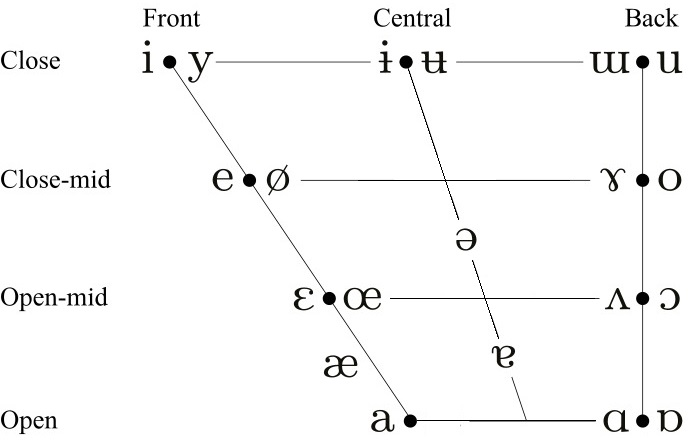
\includegraphics[width = 0.5\textwidth]{images/vowels-English.jpg}
\begin{tikzpicture}
    \tikzset
      {
        vowel/.style={circle,fill=black,minimum size=0.75ex,inner sep=0pt, outer sep=3pt},
        every label/.style={font=\strut,fill=white,outer sep=0pt, inner sep=0pt},
        titlenode/.style={font=\strut,anchor=west}
      }
      
    \node at (2,0.75) {Front};
    \node at (4,0.75) {Central};
    \node at (6,0.75) {Back};
      
    \node [titlenode] at (-1,0) {Close}; 
    \node at (2,0) [vowel, label=right:y, label=left:i] (close-front) {};
    \node at (4,0) [vowel, label=right:ʉ, label=left:ɨ] (close-central) {};
    \node at (6,0) [vowel, label=right:u, label=left:ɯ] (close-back) {};
    
    \node [titlenode] at (-1,-1) {Close-mid};
    \node at (2.5,-1)  [vowel, label=right:ø, label=left:e] (cmid-front){};
    \node at (6,-1)    [vowel, label=right:o, label=left:ɤ] (cmid-back){};
    
    \node [titlenode] at (-1,-2) {Open-mid};
    \node at (3,-2) [vowel, label=right:œ, label=left:ɛ] (omid-front) {};
    \node at (6,-2) [vowel, label=right:ɔ, label=left:ʌ] (omid-back) {};
    
    \node [titlenode] at (-1,-3) {Open};
    \node at (3.5,-3) [vowel, label=left:a] (open-front) {};
    \node at (6,-3)   [vowel, label=right:ɒ, label=left:ɑ] (open-back) {};
    
    \node [inner sep=0pt, outer sep=0pt] at (4.75,-3) (lower-border) {};
    \node [fill=white] at (4.6,-2.5) {ɐ};
    \node [fill=white] at (4.4,-1.5) {ə};
    
    
    \begin{scope}[on background layer, shorten <=8pt, shorten >=.75em]
        \draw (close-front) -- (close-central);
        \draw (close-central) -- (close-back);
        \draw [shorten >=0pt, shorten <=0pt] (close-back)  -- (open-back);
        \draw [shorten >=0pt] (open-back) -- (open-front);
        \draw [shorten >=0pt, shorten <=0pt] (open-front) -- (close-front) node [very near start, left] {æ};
        
        \draw (cmid-front) -- (cmid-back);
        \draw (omid-front) -- (omid-back);
        
        \draw [shorten >=0pt, shorten <=0pt] (close-central) -- (lower-border);
    \end{scope}
\end{tikzpicture}
\caption{Vowel space}
\label{fig:vowel-space}
\end{figure}

In this diagram, the two dimensions are height (\textit{y}-axis) and backness (\textit{x}-axis), while roundness is determined by the vowel position relative to the reference point: symbols to the left of the dot refer to unrounded vowels and those on the right are rounded.

\subsubsection{Other characteristics of vowels}

There are some other features of vowels, usually marked by diacritics or superscript symbols. For example:

\begin{itemize}
    \item Tongue root position -- can have three values:
\begin{itemize}
    \item \textsc{neutral} = the default tongue root position;
    \item \textsc{advanced} = when pronouncing the vowel, the tongue root is slightly shifted towards the front. These vowels are called ATR (advanced tongue root) and are marked in the IPA by the diacritic ◌̘;%%%%\cmubdata{◌̘};
    \item \textsc{retracted} = the tongue root is shifted towards the back (retracted). These vowels are called RTR (retracted tongue root) and are marked by ◌̙; %%%% \cmubdata{◌̙};
\end{itemize}

Generally, for languages in which the tongue root position is relevant for the vowel articulation, neutral and retracted positions are represented similarly: vowels are treated as either [+ATR] (the tongue root position is advanced) or [−ATR] (the tongue root position is neutral or retracted). Importantly, this feature of vowels is not the same as backness; there can be front [+ATR] vowels, back [+ATR] vowels, front [−ATR] vowels and back [−ATR] vowels. Moreover, this feature is often relevant to languages that display vowel harmony processes (see \sectref{sec:4-vowel-harmony}), such as many languages of Africa. In some languages, the following pairs of vowels often pattern as if they were distinguished by the feature [±ATR] (\tabref{tab:vowelsFeatureATR}).

\begin{table}[H]
  \caption{Vowels and the feature ±ATR}
  \label{tab:vowelsFeatureATR}
    \begin{tabular}{ *2{ >{[} c <{]} } }
\lsptoprule
+ATR & −ATR \\ \midrule
{u} & {ʊ} \\
{i} & {ɪ} \\
{o} & {ɔ} \\
{e} & {ɛ} \\
{a‍} & {ə} \\
\lspbottomrule
\end{tabular}
\end{table}

\item \textsc{Nasalisation} is another commonly encountered feature (present, for instance, in French and Portuguese). In the articulation of nasalised vowels, the air escapes through both the mouth and the nose. Nasalised vowels are marked by a tilde (\cmubdata{\sim}) above the vowel symbol: thus, the nasalised variant of the vowel [{o}] is [{õ}] (as in the French word \cmubdata{bon} [{bõ}]).

\item \textsc{Length} can also play an important role in some languages. It refers to the duration of the vowel and we can differentiate at least between short and long vowels (compare \textit{Ken} and \textit{cairn} in most non-rhotic English dialects or, for some speakers, the French words \textit{mettre} and \textit{maître}).\footnote{Some languages may have a three-way length distinction.} Long vowels are marked in IPA by the symbol [{ː}] placed after the vowel (this symbol is in fact made up of two triangles pointing towards one another and not by a colon. Nevertheless, in practice, the colon [{:}] is often used for simplicity). In linguistics problems, a long vowel can also be marked by doubling the vowel (thus, \cmubdata{a} is the vowel [{a}] and \cmubdata{aa} is [{aː}]) or by a bar above the vowel (\cmubdata{ā}). The same conventions can apply to long consonants, if they exist.
\end{itemize}

A final important characteristic of sounds is \textsc{syllabicity}. This denotes the ability of a sound to be the nucleus of a syllable (see below the description of syllable structure). In some languages, vowels are the only possible syllabic sounds. Nevertheless, some consonants can be syllabic in certain languages (e.g., Cantonese) and this feature is marked by a vertical line below the respective consonant (thus, syllabic \cmubdata{m} is written as [{m̩}]: consider the English interjection \textit{mmmkay} for \texttr{OK}, which we can transcribe as [{m̩.keɪ}]). We also find syllabic consonants in English words like \textit{even} [{iː.vn̩}] or \textit{rhythm} [{ɹɪ.ðm̩}]. Conversely, glides such as [{w}] and [{j}] are occasionally treated as non-syllabic versions of their respective vowels, which is signalled by an arch diacritic under the symbol: thus, [{i̯}] and [{u̯}] are broadly equivalent to [{j}] and [{w}].


\section{Syllable}

A syllable is defined as a group of sounds (phonemes) which are in some way pronounced “together”. In phonetic transcription, the boundary between syllables is marked by a full stop [{.}]: the word \textit{conclusion} can be transcribed as [{kən.kluː.ʒən}]. A syllable is comprised of three parts:

\begin{itemize}
    \item The \textsc{nucleus} is the “core”\ of the syllable: the sound occupying the nucleus is always syllabic. (This is generally what is meant when you hear that a syllable can have one and only one vowel: this is true, but as we have seen, a syllabic sound does not have to be a vowel);
    \item The \textsc{onset} represents the beginning of the syllable (everything before the nucleus);
    \item The \textsc{coda} represents the end of the syllable (everything after the nucleus).
\end{itemize}
\begin{figure}
% 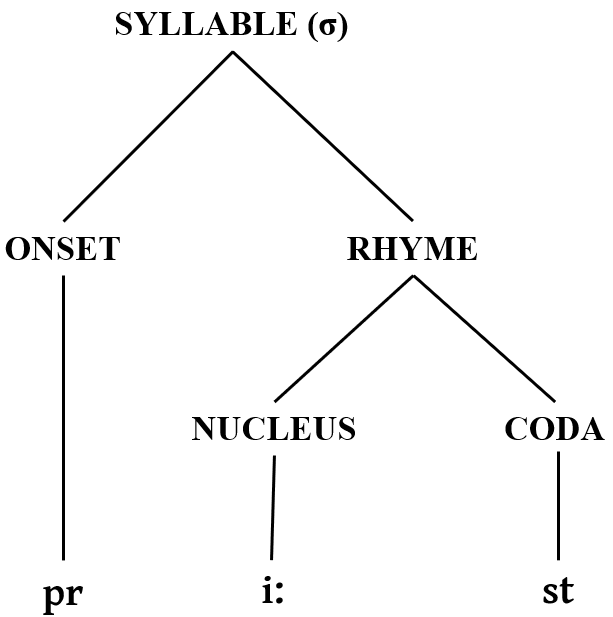
\includegraphics[width = 0.5\textwidth]{images/Syllable_EN.png}
\begin{forest}
  [Syllable (σ)
    [Onset
        [pr, tier=sound]
    ]
    [Rhyme
        [Nucleus
            [iː,tier=sound]
        ]
        [Coda
            [st,tier=sound]
        ]
    ]
  ]
\end{forest}

  \caption{Segmentation of the word \cmubdata{priest} [{pri:st}].}
  \label{fig:priest-syllable}
\end{figure}

The nucleus is the only mandatory component of a syllable: the other two are usually optional. Thus, in English, some syllables consist only of the nucleus (for example the first syllable of \cmubdata{upon} [{ə.pɒn}]), some have an onset and a nucleus but no coda (\cmubdata{me} [{mi}]), some have a nucleus and a coda but no onset (\cmubdata{at} [{æt}]), and yet others have all three (\cmubdata{cat} [{kæt}]). A further useful concept is the \textsc{rhyme}, which represents the combination of the nucleus and the coda. For example, a possible segmentation of the word \cmubdata{priest} [{pri:st}] is given in Figure \ref{fig:priest-syllable}.

\subsection{Syllabification rules}

In this subsection, we will consider the rules that we can follow in placing the syllable boundary. (For simplicity, we will not consider syllabic consonants and will only treat vowels as syllable nuclei.) A syllable generally contains only one vowel (or diphthong):\footnote{A diphthong is a group consisting of two vowel-like sounds that pattern together as if they were a single vowel, such as in \cmubdata{blind} [{bl\textbf{aɪ}nd}] or \cmubdata{lie} [{l\textbf{aɪ}}].} therefore, two consecutive vowels will always be part of two different syllables (VV \textrightarrow\ V.V).\footnote{However, remember that sequences like \cmubdata{aa} could also represent single instances of long vowels rather than two vowels in a row: check the notes for each problem!} If there is a single consonant between two vowels, this will belong to the second syllable (VCV \textrightarrow\ V.CV). This is because the basic principle of syllabification is that \textit{a consonant prefers to be an onset rather than a coda}.

Things are somewhat more complicated when there are two consonants between a vowel. One possibility is that the syllable boundary goes in the middle of the consonant “cluster”\ so that one consonant becomes the coda of the first syllable and the other becomes the onset of the second syllable (VCCV \textrightarrow\ VC.CV). In this case, the absence of consonant clusters within the syllable overrides the preference for consonants to be in an onset. Alternatively, the entire cluster can act as an onset, avoiding the coda (VCCV \textrightarrow\ V.CCV). This can also happen, but is usually the more complicated case, in that not all clusters are equally suitable for such a syllabification, so it is perhaps more prudent to assume that VCCV \textrightarrow{} VC.CV is the default pattern.

\section{Versification}

Versification problems are a special type of linguistics problem that involves a set of series of lines (verses) in a particular language, often left even without a translation. Their main purpose is determining the rules governing the structure of the verse (\textit{versification}, occasionally also \textit{prosody}, although the latter term has many other meanings). This type of problem can usually be solved using the following method:

\begin{description}[labelwidth={\widthof{Step 3.}},leftmargin=!]

\item[{Step 1.}] Syllabify all the words in each verse. A couple of issues might arise here. First, if you see two vowel symbols next to each other, make sure you know if it is a long vowel, a diphthong (a complex nucleus containing two vowel-like sounds), or a hiatus (a sequence of two vowels belonging to separate syllables). This might be explained in the footnote at the end of the problem. Second, you may need to consider whether the word boundary is relevant: sometimes each word should be syllabified on its own, but sometimes the entire verse should be treated as a single entity.

\item[{Step 2.}] Determine the type of syllable. With these problems, there are two kinds of criterion that can be used. Sometimes the relevant distinction is between syllables that contain short vowels (V) and those that contain long vowels or a diphthong (VV); sometimes, syllables without a coda contrast with those that have one; sometimes both of these criteria apply. Importantly, the onset is generally irrelevant for this type of problem.

\item[{Step 3.}] Determine the metre, that is to say, the rules regulating the kinds of syllables a verse can contain, and any restriction on their ordering. Prosodic systems generally use the criteria listed under step 2 to classify syllables as \textsc{heavy} or \textsc{light} syllables, but languages can differ in the details of this process:

\begin{itemize}\sloppy
    \item Sometimes, the distinction is solely based on the length of the vowel: light syllables have the structure (C)V(C), while heavy ones have the structure (C)VV(C);
    \item In other languages, the distinction is solely based on the existence of a coda: a syllable counts as light if it is \textsc{open}, i.e., lacks a coda and thus has the structure (C)V(V), and as heavy if it is \textsc{closed}, having the structure (C)V(V)C;
    \item In many languages, a syllable counts as heavy if it either contains a long vowel --(C)VV-- or if it is closed -- (C)V(C)C; in other words if its rhyme contains more than one element;
    \item Finally, we cannot exclude the possibility that some languages have three types of weight – light syllables (like (C)V), heavy syllables (like (C)VV or (C)VC), and superheavy syllables (like (C)VVC).
    \end{itemize}
\end{description}

 All this information is represented schematically in \figref{fig:versification}.

\begin{figure}
\caption{Versification schema.}
\label{fig:versification}
\begin{center}
%     \textbf{Legend:}

    \begin{multicols}{3}
        \begin{tabular}{c|c|}
        \cline{2-2}
             light &σ\\ \cline{2-2}
        \end{tabular}

        \begin{tabular}{c|c|}
        \cline{2-2}
             heavy & \cellcolor{lightgray}σ\\ \cline{2-2}
        \end{tabular}

        \begin{tabular}{c|c|}
        \cline{2-2}
             superheavy & \cellcolor{black} \textcolor{white}{σ} \\ \cline{2-2}
        \end{tabular}
    \end{multicols}
\end{center}

\begin{multicols}{2}
    \begin{tabular}{|c|c|c|}
        \hline 
         & short & long \\ \hline
         open &(C)V& \cellcolor{lightgray}(C)VV\\ \hline
         closed &(C)VC& \cellcolor{lightgray}(C)VVC\\ \hline
         \multicolumn{3}{c}{Type 1}\\ 
         \multicolumn{3}{c}{} \\ 
    \end{tabular}
    \begin{tabular}{|c|c|c|}
        \hline 
         & short & long \\ \hline
         open &(C)V&(C)VV\\ \hline
         closed & \cellcolor{lightgray}(C)VC& \cellcolor{lightgray}(C)VVC\\ \hline
         \multicolumn{3}{c}{Type 2}\\ 
    \end{tabular}
   \begin{tabular}{|c|c|c|}
        \hline 
         & short & long \\ \hline
         open &(C)V& \cellcolor{lightgray}(C)VV\\ \hline
         closed & \cellcolor{lightgray}(C)VC& \cellcolor{lightgray}(C)VVC\\ \hline
         \multicolumn{3}{c}{Type 3}\\ 
         \multicolumn{3}{c}{} \\ 
    \end{tabular}
    \begin{tabular}{|c|c|c|}
        \hline 
         & short & long \\ \hline
         open &(C)V& \cellcolor{lightgray}(C)VV\\ \hline
         closed & \cellcolor{lightgray}(C)VC& \cellcolor{black} \textcolor{white}{(C)VVC} \\ \hline
         \multicolumn{3}{c}{Type 4}\\
    \end{tabular}
\end{multicols}
\end{figure}

Therefore, we can certainly tell that (C)V syllables will always be light and (C)VVC will always be heavy, while the other two types can belong to either category. The final aim of the problem is to determine the structure of the verse (represented, in general, by a sequence of light and heavy syllables in a particular order). One very important thing to note is that, in many cases, there is an equivalence between one heavy syllable and two light syllables. A good indicator of this phenomenon is if the verses have a variable number of syllables.

\begin{problem}{\langnameSomali}{\nameAPiperski}{\LOYear{\IOLAbbr}{2015}}
Here are 25 half-lines of Somali poetry written in a metre known as masafo:

\begin{multicols}{2}
\begin{enumerate}[noitemsep]
    \item \cmubdata{ogaadeen ha ii dirin}
    \item \cmubdata{duul haad amxaaraa}
    \item \cmubdata{kaa dooni maayee}
    \item \cmubdata{amba waa ku daba geli}
    \item \cmubdata{dakanka iyo qaankee}
    \item \cmubdata{anaa been dabaadee}
    \item \cmubdata{galbeed uga dareershaan}
    \item \cmubdata{dalkaad adigu joogtiyo}
    \item \cmubdata{dar alliyo heshiis iyo}
    \item \cmubdata{mase waa dayoobeen}
    \item \cmubdata{dacalkaaga kuma shuban}
    \item \cmubdata{miyaan duudsiyaayaa}
    \item \cmubdata{doodaye maxaad oran}
    \item \cmubdata{daliilkii ku siiyaye}
    \item \cmubdata{miyaad iigu duurxuli}
    \item \cmubdata{dorraad adigu kama dhigin}
    \item \cmubdata{ma deldelin raggoodii}
    \item \cmubdata{deelqaadkan aad tiri}
    \item \cmubdata{diigaanyo ciidana}
    \item \cmubdata{wax ma kala dillaallaa}
    \item \cmubdata{duunyada ka qaadoo}
    \item \cmubdata{diinkiyo dugaaggiyo}
    \item \cmubdata{dildillaaca waaberi}
    \item \cmubdata{dibnahaaga kama qiran}
    \item \cmubdata{hobyo wixii ka soo degey}
    \blankitem
\end{enumerate}
\end{multicols}

To help you understand the structure of masafo, here are ten half-lines which were constructed from genuine masafo half-lines by random rearrangement of words within the half-line. Some of them might conform to the rule of versification, but the majority do not:

\begin{multicols}{2}
\begin{enumerate}[start = 26, noitemsep]
    \item \cmubdata{u anigaa lehe diin}
    \item \cmubdata{waad nimankaad ma diidi}
    \item \cmubdata{qoran daftarkaaga kuma}
    \item \cmubdata{fuushaan kaama dusha}
    \item \cmubdata{helo dabacayuun kulaan}
    \item \cmubdata{kuu miyuu tari wax dafir}
    \item \cmubdata{kuu daalasaayee nin}
    \item \cmubdata{shareecada dikrigiyo}
    \item \cmubdata{dumarkii furayaan ma}
    \item \cmubdata{ogaadee diyaar kuu}
\end{enumerate}
\end{multicols}

\begin{assgts}
\item Describe the structure of a masafo half-line.
\item Here are ten more masafo half-lines. Five of them are genuine, and five of them have been obtained by random rearrangement. Which is which?
% % \begin{multicols}{2}
\begin{enumerate}[start = 36, noitemsep]
    \item \cmubdata{war ismaaciil daarood}
    \item \cmubdata{dir miyaad wadaagtaan}
    \item \cmubdata{labadaad ka duudiye}
    \item \cmubdata{ka jannadaad daahiye}
    \item \cmubdata{adiga iyo deriskaa}
    \item \cmubdata{digaxaarka mariyoo}
    \item \cmubdata{ciid iyo doolo diraac}
    \item \cmubdata{nooma keeneen darka}
    \item \cmubdata{kala deyaayaa miyaan}
    \item \cmubdata{wuxuun kaa danqaabaan}
\end{enumerate}
% % \end{multicols}
\end{assgts}
\end{problem}

\begin{mysolution}

Firstly, we notice that there is no footnote about any of the sounds, so we can consider that there are no diphthongs and that two consecutive identical vowels (\cmubdata{aa}, \cmubdata{ii}, etc.) most likely denote a long vowel.

Next, we need to syllabify the structures. We can do that using the rules above (VV \textrightarrow\ V.V, VCV \textrightarrow\ V.CV, VCCV \textrightarrow\ VC.CV). We use a dash to mark those places where the word boundary could make a difference for the syllabification (for example, if we want to syllabify the phrase \textit{come inside} [{kʌm ɪnsaɪd}], if we are to take into account the word boundary, we would get [{kʌm ɪn.saɪd}]. However, if the word boundary is ignored, which happens quite often in rapid speech, we would get [\cmubdata{kʌ.mɪn.saɪd}]).

The verses become:

\begin{multicols}{2}
\begin{enumerate}[noitemsep]
    \item \cmubdata{o.gaa.deen.ha.ii.di.rin}
    \item \cmubdata{duul.haad-am.xaa.raa}
    \item \cmubdata{kaa.doo.ni.maa.yee}
    \item \cmubdata{am.ba.waa.ku.da.ba.ge.li}
    \item \cmubdata{da.kan.ka.i.yo.qaan.kee}
    \item \cmubdata{a.naa.been.da.baa.dee}
    \item \cmubdata{gal.beed-u.ga.da.reer.shaan}
    \item \cmubdata{dal.kaad-a.di.gu.joog.ti.yo}
    \item \cmubdata{dar-al.li.yo.hes.hii.s-i.yo}
    \item \cmubdata{ma.se.waa.da.yoo.been}
    \item \cmubdata{da.cal.kaa.ga.ku.ma-shu.ban}
    \item \cmubdata{mi.yaan.duud.si.yaa.yaa}
    \item \cmubdata{doo.da.ye.ma.xaad-o.ran}
    \item \cmubdata{da.liil.kii.ku.sii.ya.ye}
    \item \cmubdata{mi.yaad-ii.gu.duur.xu.li}
    \item \cmubdata{dor.raad-a.di.gu.ka.ma-dhi.gin}
    \item \cmubdata{ma.del.de.lin.rag.goo.dii}
    \item \cmubdata{deel.qaad.kan-aad.ti.ri}
    \item \cmubdata{dii.gaan.yo.cii.da.na}
    \item \cmubdata{wax.ma.ka.la.dil.laal.laa}
    \item \cmubdata{duun.ya.da.ka.qaa.doo}
    \item \cmubdata{diin.ki.yo.du.gaag.gi.yo}
    \item \cmubdata{dil.dil.laa.ca.waa.be.ri}
    \item \cmubdata{dib.na.haa.ga.ka.ma.qi.ran}
    \item \cmubdata{hob.yo.wi.xii.ka.soo.de.gey}
    \blankitem
\end{enumerate}
\end{multicols}

In the second verse, \cmubdata{haad-am} means that there is a word boundary between \cmubdata{haad} and \cmubdata{am}. If we ignore it, the syllables become \cmubdata{haa.dam}.

In order to simplify the problem, we can replace each syllable with the following notations (based on the syllable typology described above):

\begin{enumerate}[label = \arabic*]
    \item = syllable with short vowel and no coda = (C)V
    \item = syllable with long vowel and no coda = (C)VV
    \item = syllable with short vowel and coda = (C)VC
    \item = syllable with long vowel and coda = (C)VVC
\end{enumerate}

The corpus becomes:\largerpage[2.5]

\begin{multicols}{2}\raggedcolumns
\begin{enumerate}[noitemsep]
    \item \cmubdata{1.2.4.1.2.1.3}
    \item \cmubdata{4.haad-am.2.2}
    \item \cmubdata{2.2.1.2.2}
    \item \cmubdata{3.1.2.1.1.1.1.1}
    \item \cmubdata{1.3.1.1.1.4.2}
    \item \cmubdata{1.2.4.1.2.2}
    \item \cmubdata{3.beed-u.1.1.4.4}
    \item \cmubdata{3.kaad-a.1.1.4.1.1}
    \item \cmubdata{dar-al.1.1.3.hiis-i.1}
    \item \cmubdata{1.1.2.1.2.4}
    \item \cmubdata{1.3.2.1.1.ma-shu.3}
    \item \cmubdata{1.4.4.1.2.2}
    \item \cmubdata{2.1.1.1.xaad-o.3}\columnbreak
    \item \cmubdata{1.4.2.1.2.1.1}
    \item \cmubdata{1.yaad-ii.1.4.1.1}
    \item \cmubdata{3.raad-a.1.1.1.ma-dhi.3}
    \item \cmubdata{1.3.1.3.3.2.2}
    \item \cmubdata{4.4.kan-aad.1.1}
    \item \cmubdata{2.4.1.2.1.1}
    \item \cmubdata{3.1.1.1.3.4.2}
    \item \cmubdata{4.1.1.1.2.2}
    \item \cmubdata{4.1.1.1.4.1.1}
    \item \cmubdata{3.3.2.1.2.1.1}
    \item \cmubdata{3.1.2.1.1.1.1.3}
    \item \cmubdata{3.1.1.2.1.2.1.3}
\end{enumerate}
\end{multicols}
\pagebreak

It's time to analyse how the word boundary affects the syllable type. Let us take, for example, the structure \cmubdata{haad-am} from half-line 2.

\begin{itemize}
\item 	if we take into account the word boundary, we get: \cmubdata{haad am \textrightarrow\ haad.am (4.3)}
\item 	otherwise, we get: \cmubdata{haadam \textrightarrow\ haa.dam (2.3)}
\end{itemize}

Therefore, we notice that the only difference a word boundary makes is that a coda becomes the onset of the following syllable, so the first syllable can change from type \cmubdata{1} to \cmubdata{3} or from type \cmubdata{2} to \cmubdata{4}. The second syllable, on the other hand, is not affected in any way, because it can only receive (or lose) an onset, which, as mentioned above, is irrelevant for syllable type. If we mark the syllable before the word boundary with \cmubdata{(2/4)} or \cmubdata{(1/3)}, meaning that it can be either type \cmubdata{2} or \cmubdata{4} (or \cmubdata{1} or \cmubdata{3}, respectively), depending on whether we take into account the word boundary, and knowing that the following syllable does not change its type, we get:

\begin{multicols}{2}
\begin{enumerate}[noitemsep]
    \item \cmubdata{1.2.4.1.2.1.3}
    \item \cmubdata{4.(2/4).3.2.2}
    \item \cmubdata{2.2.1.2.2}
    \item \cmubdata{3.1.2.1.1.1.1.1}
    \item \cmubdata{1.3.1.1.1.4.2}
    \item \cmubdata{1.2.4.1.2.2}
    \item \cmubdata{3.(2/4).1.1.1.4.4}
    \item \cmubdata{3.(2/4).1.1.1.4.1.1}
    \item \cmubdata{(1/3).3.1.1.3.(2/4).1.1}
    \item \cmubdata{1.1.2.1.2.4}
    \item \cmubdata{1.3.2.1.1.(1/3)/1.3}
    \item \cmubdata{1.4.4.1.2.2}
    \item \cmubdata{2.1.1.1.(2/4).1.3}
    \item \cmubdata{1.4.2.1.2.1.1}
    \item \cmubdata{1.(2/4).2.1.4.1.1}
    \item \cmubdata{3.(2/4).1.1.1.1.(1/3).1.3}
    \item \cmubdata{1.3.1.3.3.2.2}
    \item \cmubdata{4.4.(1/3).4.1.1}
    \item \cmubdata{2.4.1.2.1.1}
    \item \cmubdata{3.1.1.1.3.4.2}
    \item \cmubdata{4.1.1.1.2.2}
    \item \cmubdata{4.1.1.1.4.1.1}
    \item \cmubdata{3.3.2.1.2.1.1}
    \item \cmubdata{3.1.2.1.1.1.1.3}
    \item \cmubdata{3.1.1.2.1.2.1.3}
    \blankitem
\end{enumerate}
\end{multicols}

Next, we notice that the number of syllables in each half-line varies between five and nine. Now recall that some versification systems make it possible to treat heavy syllables and two or more light syllables as equivalent. Nevertheless, we still need to uncover how the light and heavy syllables are defined (either light = 1, 3 and heavy = 2, 4; or light = 1, 2 and heavy = 3, 4). In order to do that, we look at the shortest (five-syllable) half-lines:

\begin{center}
\cmubdata{2.2.1.2.2} \quad\quad\quad\quad\quad \cmubdata{4.(2/4).3.2.2}
\end{center}

Since they are the shortest, we expect that they have the same structure (since there is more scope in longer verses for light syllable sequences). We can see that type \cmubdata{2} heavy syllables  ((C)VV) occur in the same positions in the verse as type \cmubdata{4} syllables ((C)VVC), whilst the type \cmubdata{1} light syllable ((C)V) matches a type \cmubdata{3} syllable ((C)VC). Therefore, we deduce that this metre features a distinction based on vowel length: light syllables are those which have a short vowel, while heavy syllables are those which have a long vowel; the presence of a coda does not make a syllable heavy. We can now rewrite all the half-lines as a sequence of light and heavy syllables, replacing \cmubdata{1} and \cmubdata{3} by L and \cmubdata{2} and \cmubdata{4} by H. We obtain the following:

\begin{multicols}{3}
\begin{enumerate}[noitemsep]
    \item L.H.H.L.H.L.L
    \item H.H.L.H.H
    \item H.H.L.H.H
    \item L.L.H.L.L.L.L.L
    \item L.L.L.L.L.H.H
    \item L.H.H.L.H.H
    \item L.H.L.L.L.H.H
    \item L.H.L.L.L.H.L.L
    \item L.L.L.L.L.H.L.L
    \item L.L.H.L.H.H
    \item L.L.H.L.L.L.L.L
    \item L.H.H.L.H.H
    \item H.L.L.L.H.L.L
    \item L.H.H.L.H.L.L
    \item L.H.H.L.H.L.L
    \item L.H.L.L.L.L.L.L.L
    \item L.L.L.L.L.H.H
    \item H.H.L.H.L.L
    \item H.H.L.H.L.L
    \item L.L.L.L.L.H.H
    \item H.L.L.L.H.H
    \item H.L.L.L.H.L.L
    \item L.L.H.L.H.L.L
    \item L.L.H.L.L.L.L.L
    \item L.L.L.H.L.H.L.L
    \blankitem
\end{enumerate}
\end{multicols}

Note that the question regarding word boundary has turned out to be irrelevant: whether we count the ambiguous consonant as a coda or not does not influence the weight of the preceding syllable.

Next, we can group the half-lines based on their number of syllables:

\vfill
\begin{table}[H]
    \begin{tabular}{cccc}
    \lsptoprule
    5 syllables & 6 syllables & 7 syllables & 8 syllables\\
    \midrule
      H.H.L.H.H &  L.H.H.L.H.H & L.H.H.L.H.L.L &   L.L.H.L.L.L.L.L\\ 
      H.H.L.H.H &  L.L.H.L.H.H & L.L.L.L.L.H.H &   L.H.L.L.L.H.L.L\\ 
                &  L.H.H.L.H.H & L.H.L.L.L.H.H &   L.L.L.L.L.H.L.L\\ 
                &  H.H.L.H.L.L & H.L.L.L.H.L.L &   L.L.H.L.L.L.L.L\\ 
                &  H.H.L.H.L.L & L.H.H.L.H.L.L &   L.L.H.L.L.L.L.L\\ 
                &  H.L.L.L.H.H & L.H.H.L.H.L.L &   L.L.L.H.L.H.L.L\\
                &              & L.L.L.L.L.H.H &                  \\
                &              & L.L.L.L.L.H.H &                  \\
                &              & H.L.L.L.H.L.L &                  \\
                &              & L.L.H.L.H.L.L &                  \\
       \lspbottomrule
    \end{tabular}
\end{table}
\vfill\pagebreak

Only one five-syllable half-line (H.H.L.H.H) seems to be possible. So, based on the above, we expect that the six-syllable half-lines can be formed by replacing one heavy syllable (H) with two light syllables (LL). Indeed, this is how most of the six-syllable half-lines can be derived. Nevertheless, two half-lines do not follow this pattern: instead, they have the structure (L.H.H.L.H.H), which is identical to that of the five-syllable half-line, but with an additional light syllable at the beginning.

Starting from the five-syllable half-line and replacing any of the heavy syllables with two light syllables (H \textrightarrow\ LL), we obtain the following possible combinations:

\begin{table}[H]
    \begin{tabular}{cccc}
    \lsptoprule
    5 syllables & 6 syllables & 7 syllables & 8 syllables\\
    \midrule
    H.H.L.H.H & L.L.H.L.H.H & L.L.L.L.L.H.H & L.L.L.L.L.L.L.H\\ 
              & H.L.L.L.H.H & L.L.H.L.L.L.H & L.L.L.L.L.H.L.L\\ 
              & H.H.L.L.L.H & L.L.H.L.H.L.L & L.L.H.L.L.L.L.L\\ 
              & H.H.L.H.L.L & H.L.L.L.L.L.H & H.L.L.L.L.L.L.L\\
              &             & H.L.L.L.H.L.L &                \\
              &             & H.H.L.L.L.L.L &                \\
    \lspbottomrule
    \end{tabular}
\end{table}

Comparing our data with the types shown in the table above, we are left with the following lines still not accounted for by the rule:

\begin{table}[H]
    \begin{tabular}{ccc}
    \lsptoprule
    6 syllables & 7 syllables & 8 syllables\\
    \midrule
    L.H.H.L.H.H & L.H.H.L.H.L.L & L.L.L.H.L.H.L.L\\
    L.H.H.L.H.H & L.H.L.L.L.H.H & L.H.L.L.L.H.L.L\\
                & L.H.H.L.H.L.L &                \\
                & L.H.H.L.H.L.L &                \\
    \lspbottomrule
    \end{tabular}
\end{table}

As previously, all the remaining six-syllable half-lines in masafo have the structure L.H.H.L.H.H, equivalent to a five-syllable half-line with an extra light syllable in the beginning. Furthermore, all the remaining seven- and eight-syllable half-lines are also formed by replacing one or two heavy syllables in this type of six-syllable structure with light syllables (H \textrightarrow\ LL).

The only half-line we have not analysed so far is the nine-syllable one, which has the structure L.H.L.L.L.L.L.L.L. We notice that this one is also derived from the same six-syllable half-line: 

\begin{center}
L.H.L.L.L.L.L.L.L \Leftrightarrow\ L.H.(L.L).L.(L.L).(L.L) \Leftrightarrow\ L.H.H.L.H.H.
\end{center}

We can therefore deduce that all half-lines in the masafo metre derive from either H.H.L.H.H or L.H.H.L.H.H. This can also be written as (L).H.H.L.H.H, in which any of the heavy syllables (H) can be replaced by two light syllables (LL).

Of course, there are other approaches which yield the same result. For example, we can notice that most half-lines end in two heavy syllables; where this is not the case, we always have a heavy syllable followed either by two light syllables or just by four light syllables. We discover that all half-lines end with H.H (where each H can be replaced by L.L). Excluding these syllables, we are left with:

\begin{table}[H]
    \begin{tabular}{ccccc}
    \lsptoprule
        5 syllables & 6 syllables & 7 syllables & 8 syllables & 9 syllables\\
    \midrule
        H.H.L & L.H.H.L &   L.H.H.L   &   L.L.H.L   &    L.H.L.L.L\\
        H.H.L & L.L.H.L &   L.L.L.L.L &   L.H.L.L.L &             \\
              & L.H.H.L &   L.H.L.L.L &   L.L.L.L.L &             \\
              & H.H.L   &   H.L.L.L   &   L.L.H.L   &             \\
              & H.H.L   &   L.H.H.L   &   L.L.H.L   &             \\
              & H.L.L.L &   L.H.H.L   &   L.L.L.H.L &             \\
              &         &   L.L.L.L.L &             &             \\
              &         &   L.L.L.L.L &             &             \\
              &         &   H.L.L.L   &             &             \\
              &         &   L.L.H.L   &             &             \\    
    \lspbottomrule
    \end{tabular}
\end{table}

Next, we notice that all half-lines end in a light syllable. Excluding this syllable as well, we get the following table. Note that we removed all duplicate structures (i.e., if, for example, all five-syllable verses remained with the structure H.H, we only included it once in the table:

\begin{table}[H]
    \begin{tabular}{ccccc}
    \lsptoprule
        5 syllables & 6 syllables & 7 syllables & 8 syllables & 9 syllables\\
    \midrule
        H.H & L.H.H & L.H.H   &    L.L.H & L.H.L.L\\
            & L.L.H & L.L.L.L &  L.H.L.L &        \\
            & H.H   & L.H.L.L &  L.L.L.L &        \\
            & H.L.L & H.L.L   &  L.L.L.H &        \\
            &       & L.L.H   &          &        \\
    \lspbottomrule
    \end{tabular}
\end{table}
    
Repeating the same thought process we notice, again, that most half-lines end in two heavy syllables or their equivalent (that is, L.L.L.L or H.L.L or L.L.H). If we also exclude these, we get:

\begin{table}[H]
    \begin{tabular}{cccc}
    \lsptoprule
        6 syllables & 7 syllables & 8 syllables & 9 syllables\\
    \midrule
         L & L & L & L\\
     \lspbottomrule
    \end{tabular}
\end{table}

Now we are left (only in some half-lines) with a light syllable in the beginning; we infer that this syllable is optional.

Both approaches yielded the same result: the structure of a masafo half-line is (L).H.H.L.H.H, where H can be replaced by L.L; H represents a heavy syllable (with a long vowel), while L represents a light syllable (with a short vowel).

In order to solve task (b), we need to follow the same algorithm: syllabification and marking the syllables as L or H. We get:

\begin{multicols}{2}
\begin{enumerate}[start = 36, noitemsep]
    \item L.L.H.H.H.H
    \item L.L.H.L.H.H
    \item L.L.H.L.H.L.L
    \item L.L.L.H.H.L.L
    \item L.L.L.L.L.L.L.H
    \item L.L.H.L.L.L.H
    \item H.L.L.H.L.L.H
    \item H.L.H.H.L.L
    \item L.L.L.H.H.L.H
    \item L.H.H.L.H.H
\end{enumerate}
\end{multicols}

We already know that each half-line needs to end in two heavy syllables (or the equivalent with light syllables), and this needs to be preceded by a light syllable (L.H.H /L.L.L.H/L.H.L.L/ L.L.L.L.L), so we can easily figure out that the half-lines 36, 39, 42, 43, and 44 are not genuine. Since we are told that exactly five of them are not genuine, we know for sure that the rest are genuine.
\end{mysolution}

\section{Stress}

In another type of linguistics problem based solely on phonetic concepts, we are given some words with the stress marked and asked to identify the pattern of stress placement and apply it to other words. Roughly, a stressed syllable is pronounced with more emphasis, allowing us to differentiate between, e.g., \cmubdata{\textbf{con}trast} (stress on \cmubdata{con}, as in the noun) and \cmubdata{con\textbf{trast}} (stress on \cmubdata{trast}, as in the verb). The stress can also be marked by a prime symbol before the relevant syllable.\footnote{For example, in the IPA notation, the phonetic transcription of the two words would be [{ˈkɒn.trɑːst}] and [{kən.ˈtrɑːst}], respectively.} This stress is also called \textit{primary} stress and, by definition, each word only contains one syllable with a primary stress.

From a typological perspective, some languages have fixed stress and others have mobile (or variable) stress. For those which have fixed stress, the stress is usually placed towards the edge of the word (either the beginning or the end). Therefore, there are languages in which the primary stress always falls on the last syllable and languages in which stress always falls on the first syllable. Alternatively, there are languages in which stress always falls on the second or penultimate syllable or even the third or antepenultimate syllable. Generally, the first and last three syllables of a word are the most likely stress positions.

\begin{sloppypar}
Languages which have variable stress can be further subdivided into two classes: languages with “free”\ stress and languages with “predictable”\ stress. By free stress is meant that on a word-by-word basis you cannot predict the stress pattern (but each word will have a fixed pattern). In languages with “predictable”\ stress, the stress placement follows some well-defined rules, usually related to the weight of syllables. In linguistics problems, we usually find languages with predictable stress, because free stress cannot be predicted, while fixed stress is extremely easy to analyse.
\end{sloppypar}

In the case of languages with predictable stress, stress is usually placed within a \textit{window}\ (i.e., a group of syllables, with the accent always falling on one of these syllables, based on certain rules). The most common stress windows are the first and the last three syllables and, within these windows, certain rules dictate stress placement, which are often similar to the rules in versification problems. For instance, stress could always fall on the syllable that contains a long vowel (within a certain stress window), and, if there is no such syllable, it will be placed on the first syllable within that window. Generally, all these rules are based on syllable weight (i.e., vowel length and/or the presence of a coda). It is possible, but rare, for stress placement to also be determined by factors such as the quality of the vowel (front/back, open/close, etc.).

To give you an idea of how complex such systems can be, let us consider the case of the Pirahã language.\footnote{This phenomenon was featured in a problem by \nameASemenuks\ (IOL 2013).} In this language, the stress window is represented by the final three syllables (thus, the primary stress will always be placed on one of the last three syllables). The placement of the stress is determined by a hierarchy of syllable types that takes into account both the type of vowel (long or short) and the \OlympiadNewTerm{type of onset} (an extremely rare thing). Specifically, syllables with a long vowel are always higher in the hierarchy (``heavier") than those with a short vowel, while syllables that feature a voiceless onset are higher than those that have a voiced onset (which are themselves higher than those which have no onset). If we denote a voiced consonant as G and a voiceless consonant as C (and, as previously, use V for a short vowel and VV for a long vowel or diphthong), the syllable hierarchy in Pirahã is: CVV > GVV > VV > CV > GV > V. Furthermore, if there are several syllables of the same type within the window, stress will be placed on the rightmost syllable (last > penultimate > antepenultimate). For example, in the word [{ka.gi.hi}] \texttr{wasp}\ we have two CV syllables ([ka] and [hi]) and one GV syllable ([gi]]. We know that CV syllables have priority, so, certainly, the stress will not be placed on [gi]. Amongst the remaining two syllables (which are of the same type), the stress will be placed on the rightmost syllable, so the word is stressed [ka.gi.ˈhi].

By contrast in [ʔi.soo.bai] \texttr{otter}\ stress goes on [soo]: it has priority over the first syllable since it has a long vowel and it also has priority over the last syllable since it has a voiceless onset.

Apart from primary stress, some languages can also have \textit{secondary} stresses. These are also marked with a prime symbol, but placed below the line (\,ˌ\,). There is no limit as to how many secondary stresses a word can have and usually the rules for placing the secondary stress are based on the type of syllable or vowel (e.g., all syllables with a long vowel that do not bear primary stress will receive secondary stress) or related to the primary stress (e.g., starting from the primary stress towards the right, every other syllable receives secondary stress).

\begin{problem}{\langnameManobo}{\nameSVaduguru}{\LOYear{\PLOAbbr}{2020}}
Given below are some words in Sarangani Manobo. In each word, the location of the stress is marked with \cmubdata{ˈ} at the beginning of the stressed syllable:

\begin{exe}\sloppy
  \sn[]{\cmubdata{ˈbaso}, \cmubdata{deˈitek}, \cmubdata{meneˈnoo}, \cmubdata{beˈgas}, \cmubdata{leˈkat}, \cmubdata{ˈotaw}, \cmubdata{eteˈbay}, \cmubdata{bineleˈsan}, \cmubdata{ˈdeget}, \cmubdata{ˈbenget}, \cmubdata{miˈneles}, \cmubdata{ˈikan}, \cmubdata{ˈdoen}}
\end{exe}

\begin{assgts}
\item Mark the stress in the following words:
\begin{multicols}{2}
\noindent 
    \begin{itemize}
    \item[] \cmubdata{mengabat}
    \item[] \cmubdata{tadon}
    \item[] \cmubdata{migbasa}
    \item[] \cmubdata{belegkong}
    \item[] \cmubdata{iselem}
    \item[] \cmubdata{mola}
    \item[] \cmubdata{benal}
    \item[] \cmubdata{medaet}
    \end{itemize}
\end{multicols}

\item Given a new word in Sarangani Manobo, how would you identify the syllables in the word? Once you have identified the syllables, how would you determine which syllable is stressed?
\end{assgts}
\end{problem}

\begin{mysolution}

Syllabification has already been discussed above; we can apply the usual rules (VV \textrightarrow\ V.V, VCV \textrightarrow\ V.CV, VCCV \textrightarrow\ VC.CV).

The first step is to notice where the stress is usually placed. We know it is most likely placed in a window either at the beginning or at the end of the word. Looking at the word \cmubdata{bineleˈsan}, we infer that, most likely, the stress window is at the end of the word; if it were in the beginning, it would be four syllables long, which is unlikely. Assuming the stress window is at the end of the word, we notice that the stress can only fall on the last or penultimate syllable.

The next step is splitting the words into two groups, based on the stress position:

\begin{table}[H]
    \begin{tabular}{ll}
    \lsptoprule
    Penultimate syllable & Final syllable \\ \midrule
    \cmubdata{ˈba.so}     & \cmubdata{bi.ne.le.ˈsan} \\
    \cmubdata{ˈde.get}    & \cmubdata{e.te.ˈbay} \\
    \cmubdata{ˈben.get}   & \cmubdata{le.ˈkat} \\
    \cmubdata{mi.ˈne.les} & \cmubdata{be.ˈgas} \\
    \cmubdata{ˈi.kan}     & \cmubdata{me.ne.ˈnoo} \\
    \cmubdata{ˈdo.en}     &                       \\
    \cmubdata{ˈo.taw}     &                       \\
    \cmubdata{de.ˈi.tek}  &                       \\
    \lspbottomrule
    \end{tabular}
\end{table}

Since most of the words have the stress placed on the penultimate syllable, we can assume that this is the default position and, in some cases, the stress shifts to the last syllable. The first hypothesis is that the stress moves to the last syllable if it contains a long vowel (\cmubdata{me.ne.ˈnoo}), but this is the only word that contains a long vowel: such a rule is unlikely to help us with the task. Another idea to consider is that all words in which the stress is on the last syllable end in a closed syllable (with a coda) and furthermore in all these cases the penultimate syllable is open (lacks a coda). Therefore, we could hypothesise that the stress falls, in general, on the penultimate syllable, and moves to the last syllable if the latter is closed whilst the penultimate syllable is open. This hypothesis is also quickly rejected since we have words such as \cmubdata{de.ˈi.tek} and \cmubdata{ˈo.taw} in which the penultimate syllable is open and the last syllable is closed, but the stress still falls on the penultimate syllable.

Therefore, vowel length and syllable type seem to not play an important role in stress placement. Looking at the type of vowel, we notice that all words in which the stress falls on the last syllable contain the vowels \cmubdata{a} or \cmubdata{o}. Perhaps stress prefers a syllable that contains these two vowels? However, this also proves to be wrong since we have words such as \cmubdata{ˈi.kan}.

Up until now, we have tried finding a reason for stress to move to the last syllable rather than the penultimate (that is, stress is \emph{attracted} to the final syllable by virtue of some property of that syllable, such as a long vowel, coda, or the vowels \cmubdata{a} or \cmubdata{o}). Perhaps, instead, it is the opposite: could stress actually be \emph{repulsed} from the penultimate syllable to the last one in some contexts? We can observe that in all words with stress on the last syllable, the penultimate syllable contains the vowel \cmubdata{e}. Therefore, we need to consider the hypothesis that stress prefers to be on a syllable that does not contain the vowel \cmubdata{e}.

We can try and classify the words based on the presence of the vowel \cmubdata{e} in the last or penultimate syllable:

\begin{table}[H]
     \begin{tabular}{lll}
     \lsptoprule
                   & \multicolumn{2}{c}{Penultimate syll.} \\\cmidrule(lr){2-3}
        Last syll. & V=\cmubdata{e} & V\neq \cmubdata{e} \\ \midrule
        V=\cmubdata{e} & \cmubdata{ˈdeget}   & \cmubdata{deˈitek}\\ 
                       & \cmubdata{ˈbenget}  & \cmubdata{ˈdoen}  \\
                       & \cmubdata{miˈneles} &                   \\
       \addlinespace     
        V\neq \cmubdata{e} &  \cmubdata{meneˈnoo}   & \cmubdata{ˈbaso} \\
                           &  \cmubdata{beˈgas}     & \cmubdata{ˈotaw} \\
                           &  \cmubdata{leˈkat}     & \cmubdata{ˈikan} \\
                           &  \cmubdata{eteˈbay}    &                  \\
                           &  \cmubdata{bineleˈsan} &                  \\
     \lspbottomrule
     \end{tabular}
\end{table}

We notice that if only one of the last two syllables contains the vowel \cmubdata{e}, stress is placed on the other syllable. If both syllables contain the vowel \cmubdata{e}, stress falls on the penultimate syllable; the same happens if none of them contains the vowel \cmubdata{e}. Alternatively, we can describe the situation thus: stress falls on the last syllable only if it does not contain the vowel \cmubdata{e} and the penultimate syllable does. An even simpler way of formulating the rule is that stress is placed on the penultimate syllable, but is repulsed to a final syllable by the vowel \cmubdata{e}. Therefore:

\begin{itemize}
    \item if none of the vowels is \cmubdata{e}, the stress remains in the default position, the penultimate syllable;
    \item if the last vowel is \cmubdata{e}, the stress stays in the default position, on the penultimate syllable;
    \item if the penultimate vowel is \cmubdata{e}, the stress is forced to move to the last syllable. We have two cases:
    \begin{itemize}
        \item if the last vowel is not \cmubdata{e}, the stress will favour this position and will remain on the last syllable;
        \item if the last vowel is also \cmubdata{e}, the stress cannot fall on it either, so it will stay on the penultimate syllable since this is the default position.
    \end{itemize}
\end{itemize}

Finally, if we return to the only example featuring a long vowel, \cmubdata{me.ne.ˈnoo}, we notice that there is an alternative explanation: \cmubdata{oo} is not a long vowel, but rather two short, independent vowels and the syllabification of the word is, in fact, \cmubdata{me.ne.ˈno.o}. Either way, the stress rule is followed. Since there is only one example of a double vowel and there is no footnote explaining its role, we can simply assume that there are two short vowels.

Thus, we can solve the two tasks:

\begin{solutions}
    \item \begin{itemize}[leftmargin = 1em]

    \begin{multicols}{4}
        \item[] \cmubdata{men.ˈga.bat}
        \item[] \cmubdata{mig.ˈba.sa}
        \item[] \cmubdata{i.ˈse.lem}
        \item[] \cmubdata{be.ˈnal}
        \item[] \cmubdata{ˈta.don}
        \item[] \cmubdata{be.leg.ˈkong}
        \item[] \cmubdata{ˈmo.la}
        \item[] \cmubdata{me.ˈda.et}
    \end{multicols}
    \end{itemize}
    \item For syllabification, we use the rules:
    \item[] \quad\quad VV \textrightarrow{} V.V\hfill VCV \textrightarrow{} V.CV\hfill VCCV \textrightarrow{} VC.CV
    \item[] Stress falls on the penultimate syllable. If it contains the vowel \cmubdata{e} (and the last syllable does not), stress will move to the last syllable.
\end{solutions}
\end{mysolution}

\section{Tone}\label{sec:3.6}\largerpage

Another phonetic phenomenon is \emph{tone}. This term covers the use of \emph{pitch} to make distinctions in the meaning of words, and/or grammatical distinctions.

Technically, pitch is the frequency with which the vocal folds vibrate in the production of speech, also known as the \emph{fundamental frequency} (for this reason, only voiced sounds are characterised by pitch). Most, if not all, languages make some use of pitch. For example, in many languages syllables that carry stress are characterised by a higher pitch than unstressed ones: most varieties of English belong to this type. In some languages, such as for example Russian, the pitch trajectory is the only difference between a statement and a general question, in contrast to, say, English, which uses a special construction to distinguish between \textit{You solved the problem} and \textit{Did you solve the problem?}

Such uses of pitch are found in many languages of the world, and are covered by the label \emph{intonation}. The term tone is narrower: we say that a language is a \textit{tone language} if tone can make lexical or grammatical distinctions between words. For example, the syllable \cmubdata{ma} in Mandarin can have different meanings depending on the tone it receives (as we have seen in the previous chapter). As such, the word \cmubdata{mā}, with first tone, means \texttr{mother}, while the word \cmubdata{má} (second tone) means \texttr{hemp}, \cmubdata{mǎ} (third tone) means \texttr{horse}, and \cmubdata{mà} (fourth tone) means \texttr{scold}.

In such cases, tonal differences are not really different from distinctions made using, say, two different consonants. There are also languages where changes in tone can express grammatical meanings, similar to how such meaning can be expressed by a morpheme (see \chapref{chap-noun} for more information about morphemes).

The terminology used for tone languages can differ quite a lot, so you may need to read the pronunciation notes carefully to make sure you understand the notation in the problem.

Tone, like stress, is an example of a \emph{suprasegmental} phenomenon. Whilst properties such as, say, backness or place of articulation belong only to the vowel or consonant they are associated with, suprasegmental features characterise groups of consonants and vowels (collectively called \textit{segments}). With stress, we saw that it is mostly a property of syllables, and this is often the case also with tone. 
% Very occasionally, you might come across other suprasegmental properties, which can be expressed phonetically using parameters such as \emph{voice quality}. An example is \emph{creaky voice}, which many English speakers refer to as `vocal fry': there are languages where creaky voice quality is distinctive just like pitch height.

\hypertarget{practice-problems}{%
\section{Practice problems}}
\largerpage
\begin{problem}{Old Javanese}{\nameMSalter}{\LOYear{\UKLOAbbr}{2021}}
The Kakawin poems of Old Javanese were long narrative tales made up of four-line stanzas. In the tradition of early Sanskrit poetry, each line was made up of a precise pattern of heavy and light syllables. The first section of the 11th-century CE Kakawin poem \textit{Arjunawiwāha} (‘The Marriage of Arjuna’) consisted of lines which followed the \textit{śārdūlawikrīdita} metre. In this metre, all lines have the same pattern: each consists of 19 syllables in an exact pattern of heavy and light syllables, except for the last syllable which can be either heavy or light. The first three syllables of a \textit{śārdūlawikrīdita} line are all heavy.

Below are two stanzas from the opening section of the \textit{Arjunawiwāha}:

\begin{enumerate}[noitemsep]
    \item \cmubdata{lakṣmī niŋ suraloka sampun ayaśâŋrĕñcĕm tapa mwaŋ brata}
    \item[] \cmubdata{akweh saŋ pinilih pituŋ siki tikāŋ antuk niŋ okir mulat}
    \item[] \cmubdata{rwêkāŋ ādi Tilottamā pamĕkas iŋ kocap lawan Suprabā}
    \item[] \cmubdata{tapwan marma tuhun lĕhĕŋ lĕhĕŋa saŋkê rūpa saŋ hyaŋ Ratih}
    \item[]
    \item \cmubdata{tambenyân liniŋir kĕtêkin inamĕr deniŋ watĕk dewata}
    \item[] \cmubdata{sampūrna pwa ya mapradakṣina ta yâmūjâmidĕr pintiga}
    \item[] \cmubdata{hyaŋ Brahmā dumadak caturmuka batārêndrâmahâkweh mata}
    \item[] \cmubdata{eraŋ miŋgĕka kociwâmbĕk ira yan kālanyan uŋgw iŋ wuri}
\end{enumerate}

\begin{assgts}
\item Here are four more lines from the first section of the \textit{Arjunawiwāha} (in the \textit{śārdūlawikrīdita} metre), with their component parts (labelled A–D) \OlympiadRandomOrder{}: 
{\columnsep=-5pt%
\begin{multicols}{2}\raggedcolumns
\begin{enumerate}[label = Verse \arabic*:, start=1, align=left, leftmargin=*]
\item 
\begin{enumerate}[label = Part \Alph*:, start = 1, align=left, labelsep=\widthof{~}, leftmargin=-12pt]
    \item[]
    \item \cmubdata{yêkā rakwa}
    \item \cmubdata{kapwa tâmurṣita}
    \item \cmubdata{Indra sĕdĕŋ amwit}
    \item \cmubdata{kinon hyaŋ}
\end{enumerate}

\item
\begin{enumerate}[label = Part \Alph*:, start = 1, align=left, labelsep=\widthof{~}, leftmargin=-12pt]
    \item[]
    \item \cmubdata{daśagunan}
    \item \cmubdata{tan sora}
    \item \cmubdata{pwa tĕkap nikā}
    \item \cmubdata{rūpanya dentânaku}
\end{enumerate}
\columnbreak
\item
\begin{enumerate}[label = Part \Alph*:, start = 1, align=left, labelsep=\widthof{~}, leftmargin=-12pt]
    \item[]
    \item \cmubdata{widyādarī mūr tĕhĕr}
    \item \cmubdata{sinambahakĕn iŋ}
    \item \cmubdata{liŋ hyaŋ}
    \item \cmubdata{Śakra nahan}
\end{enumerate}

\item
\begin{enumerate}[label = Part \Alph*:, start = 1, align=left, labelsep=\widthof{~}, leftmargin=-12pt]
    \item[]
    \item \cmubdata{lokika}
    \item \cmubdata{tan sangkêŋ}
    \item \cmubdata{lwir saŋgrahêŋ}
    \item \cmubdata{wiṣaya prayojñananira}
\end{enumerate}
\end{enumerate}
\end{multicols}}

\item[] For each verse, place the parts A-D in the right order to obtain the original verse.
\item Below are given four more words which appear in different lines from the first section of the \textit{Arjunawiwāha}:\largerpage

\begin{multicols}{2}
\begin{itemize}
    \item[] \cmubdata{paramārthapandita}
    \item[] \cmubdata{ametmetâśrayā}
    \item[] \cmubdata{santosâhĕlĕtan}
    \item[] \cmubdata{candanâpāyunan}
\end{itemize}
\end{multicols}

\item[] For each of them, write the number (from 1 to 19) of the syllable in their respective lines of which these words begin (e.g., 1 if the word is at the start of the line, 3 if the word's first syllable is the third in the line).
\end{assgts}

\begin{tblsWarning}
\cmubdata{ā}, \cmubdata{â}, \cmubdata{ê}, \cmubdata{ĕ}, \cmubdata{ī}, \cmubdata{ū} are vowels. \cmubdata{ŋ}, \cmubdata{ñ}, \cmubdata{ṣ}, \cmubdata{y} are consonants. You should assume that long vowels \cmubdata{ā}, \cmubdata{ī}, \cmubdata{ū} (and possibly others) occur only in heavy syllables. 
\end{tblsWarning}
\end{problem}

\begin{problem}{\langnameChuvash}{\nameASemenuks}{\LOYear{\LLOAbbr}{2013}}
Here are some Chuvash words, transcribed in Latin script. The stress is marked by a prime symbol before the respective syllable.

\begin{center}

\begin{tabular}{ll@{\hskip0.5in}ll}
     \pbsv{aˈvallăh}{antiquity}& \pbsv{malašneˈhi}{future} \\
     \pbsv{asărhaˈnullă}{sensitive}& \pbsv{mĕskĕnˈlen}{to respect} \\
     \pbsv{ănsărˈtran}{unexpected}& \pbsv{nušalanˈtar}{to make suffer} \\
     \pbsv{ˈăšăn}{to warm up}& \pbsv{ˈpĕlĕtlĕ}{cloudy} \\
     \pbsv{ˈvărlăh}{seed}& \pbsv{ˈpitĕrĕnčĕk}{closed} \\
     \pbsv{ˈĕmĕrlĕh}{for life}& \pbsv{suˈnarșă}{hunter} \\
     \pbsv{jüˈșek}{sour, bitter}& \pbsv{čuˈralăh}{slavery} \\
     \pbsv{kansĕrˈle}{to trip}& \pbsv{čuhănˈlan}{to become poor} \\
     \pbsv{kĕrkunieˈhi}{autumn}& \\
\end{tabular}
\end{center}
\begin{assgts}
\item Mark the stress in the following words:

\begin{tabular}{ll@{\hskip0.5in}ll}
     \pbsv{vĕltrentărri}{tit (bird)}& \pbsv{jyvărlăh}{difficulty} \\
     \pbsv{vișmine}{overmorrow}& \pbsv{măkărălčăk}{convex} \\
     \pbsv{ilĕrtüllĕ}{tempting}&  \\
\end{tabular}
\end{assgts}

\begin{tblsWarning}
\cmubdata{ă} and \cmubdata{ĕ} are extra-short vowels, which are pronounced shorter than the other vowels in the language. \cmubdata{ü} and \cmubdata{y} are vowels; \cmubdata{ș}, \cmubdata{š} and \cmubdata{č} are consonants.
\end{tblsWarning}
\end{problem}

\begin{problem}{\langnameAncientGreek}{\nameDMirea}{\LOYear{\RoLOAbbr}{2019}}
In Ancient Greece, poetry was the most celebrated art. There were several poetic forms, each with its own rules of rhythm, metre and rhyme. In order to describe these forms, the Greeks established the art of prosody, regulating the structure of verses. In this problem, you will decipher the structure of some poems of Ancient Europe. 

A metrical foot is a sequence of short (\cmubdata{S}) and long (\cmubdata{L}) syllables repeated in a verse. A line consists of several feet, as in the following example:
\begin{center}
\cmubdata{L-S-X | L-S-X | L-S-X}    
\end{center}

The verse above contains nine syllables and three metrical feet. The metrical foot, in this case, is formed by three syllables \cmubdata{L-S-X}, where \cmubdata{X} is a syllable that can be either short or long. All the verses of a poem written in this metre will have the same structure. In Ancient Greek, a syllable counts as long if it contains a long vowel or a diphthong, or if it ends in a consonant. Syllabification does not necessarily take into account word boundaries. 

Below are eight verses, transliterated into Latin script, from \textit{Oedipus Tyrannus} (or \textit{Oidipous Tūrannos}, in Ancient Greek), Sophocles' tragedy. These are written in the most common metre at that time. The number after the verse represents the verse's number in the original work.

\begin{table}[H]
\begin{tabular}{l@{\hskip1em}r}
\cmubdata{ō tekna, Kadmou tou palai neā tropʰē,} &(1) \\
\cmubdata{tinas potʰ' edrās tāsde moi tʰoazdetē} &(2)\\
\cmubdata{ʰiktēriois kladoisin eksestemmenoi;}	&(3) \\
\cmubdata{polis d' ʰomou men tʰūmiāmatōn gemei,}	&(4) \\
\cmubdata{ʰomou de paianōn te kai stenagmatōn.}	&(5) \\
\cmubdata{ēn ʰēmin, ōnaks, Lāïos potʰ' ʰēgemōn}	&(103) \\
\cmubdata{poion logon; leg' autʰis, ōs māllon matʰō} &(358) \\
\cmubdata{oukʰi ksunēkas prostʰen; ʰē 'kpeirā legōn;} &(359)
\end{tabular}
\end{table}

\begin{assgts}
\item Describe the syllabification rules and the structure of the metre in \textit{Oedipus Tyrannus}. How many metrical feet does a verse have? 
\item The following four verses were written by other important writers of Ancient Greek. Only one of them is written in the same metre as that of Sophocles. Which one is it? 

  \begin{exe}
    \sn[]{
    (Aeschylus, \textit{Prometheus bound}, 543)  \\
    \cmubdata{tʰeit' ema gnōmā kratos antipalon Zeus}}
    
    \sn[]{
    (Aristophanes, \textit{The clouds}, 609)  \\
    \cmubdata{prōta men kʰairein Atʰēnaioisi kai tois...}}
    
    \sn[]{
    (Euripides, \textit{Hippolytus}, 1054)  \\
    \cmubdata{ei pōs dunaimēn, ōs son ekʰtʰairō karā.}}
    
    \sn[]{
    (Herodas, \textit{Mimiamb}, 14)  \\
    \cmubdata{o pēlos akʰris ignuōn prosestēken:}}
  \end{exe}


\item Latin civilization perpetuated many aspects of Greek culture. In particular, the metre used by Sophocles and other Greek writers was later taken over and adapted by Latin writers. The following excerpt is from \textit{Medea}, the tragedy by Seneca. The verse structure is identical to that of Sophocles, but one of the feet presents a slight modification. What is the modification and in which foot is it?
\begin{center}
\begin{tabular}{l@{\hskip1em}l}
    \cmubdata{Lūcīna, custos, quaeque domitūram fretī} &(2) \\
    \cmubdata{Tiphyn nouam frēnāre docuistī ratem…} &(3)\\
\end{tabular}
\end{center}
\end{assgts}

\begin{tblsWarning} 
In Ancient Greek, \cmubdata{ai}, \cmubdata{oi}, \cmubdata{ei}, \cmubdata{au}, \cmubdata{eu}, \cmubdata{ou} are diphthongs; \cmubdata{pʰ}, \cmubdata{tʰ} and \cmubdata{kʰ} are consonants. \cmubdata{ʰ} before a vowel shows that it is preceded by a puff of air similar to \texttr{h}. Treat sequences of a vowel and \cmubdata{i} as diphthongs, unless the \cmubdata{i} appears as \cmubdata{ï}, in which case it forms its own syllable. The apostrophe \cmubdata{'} marks a vowel that has been deleted (or elided).

In Latin, \cmubdata{qu} is a single consonant pronounced like \texttr{c} followed by \texttr{w}; \cmubdata{ph} and \cmubdata{f} are pronounced the same as each other, \cmubdata{y} is a vowel, \cmubdata{ae} is a diphthong. \cmubdata{u} between two vowels behaves like a consonant. 

The mark {\char"25CC\char"304} above a vowel denotes length. %%% \fbox{\cmubdata{¯}}
\end{tblsWarning}
\end{problem}
\pagebreak

\begin{problem}{\langnameFijian}{\nameRDinca}{\LOYear{\RoLOAbbr}{2015}}
Here are some words in Fijian, with the primary and secondary stresses marked:

\begin{exe}\sloppy
\sn[]{\cmubdata{láko}, \cmubdata{paràimarí:}, \cmubdata{tálo}, \cmubdata{βináka}, \cmubdata{kilá:}, \cmubdata{nrè:nré:}, \cmubdata{atómi}, \cmubdata{perèsiténdi}, \cmubdata{mìnisìterí:}, \cmubdata{mbàsikètepólo}, \cmubdata{mbè:léti}, \cmubdata{Seŋái}, \cmubdata{taràusése}, \cmubdata{parò:karámu}, \cmubdata{mì:sìniŋgáni}, \cmubdata{ndàirèkitá:}}
\end{exe}

\begin{assgts}
\item Mark the primary and secondary stresses in the following words:
\begin{center}
\cmubdata{mbelembo:tomu}, \cmubdata{mbasa:}, \cmubdata{ndikonesi}, \cmubdata{ndoketa:}, \cmubdata{palasita:}, \cmubdata{terenisisita:}
\end{center}
\end{assgts}

\begin{tblsWarning} 
The marks {\char"25CC\char"300} and {\char"25CC\char"301} above a vowel mark the primary and secondary stress, respectively. Two consecutive vowels form a diphthong. The mark \cmubdata{:} after a vowel denotes length.
\end{tblsWarning}
\end{problem}

\begin{problem}{\langnameOldNorse}{\namePArkadiev\ \& \nameEGurevich}{\LOYear{\MSKAbbr}{2006}}
A professor of Old Norse philology, while explaining to his students the principles of Old Icelandic versification, invited them to analyse several lines from an Old Icelandic manual on versification written in the 13th century, containing lists of the names of mythological characters and objects, sometimes connected with each other by the word \cmubdata{ok} (\texttr{and}). Below are these few lines and the professor's instructions to the students. There are some gaps in the instructions. 

\begin{enumerate}[label = A\arabic*., leftmargin = 1in]
    \item \cmubdata{Randverr, Rökkvi, || Reifnir, Leifnir}
    \item \cmubdata{Gaurekr ok Húnn, || Gjúki, Buðli}
    \item \cmubdata{Þórr ok Hildolfr, || Hermóðr, Sigi}
    \item \cmubdata{Byrvill, Kílmundr, || Beimi, Jórekr}
    \item \cmubdata{Svalinn ok Randi, || Saurnir, Borði}
    \item \cmubdata{Hildr ok Skeggöld, || Hrund, Geirdriful}
    \item \cmubdata{Viðarr ok Baldr, || Váli ok Heimdallr}
    \item \cmubdata{Frigg ok Freyja, || Fulla ok Snotra}
    \item \cmubdata{Skávær, Skáviðr, || Skirfir, Virfir}
\end{enumerate}

The professor's instructions:
\begin{quote}
    In Old Icelandic versification, the main poetic technique is alliteration, i.e., the repetition of the initial sounds of words. You need to know the following about Old Icelandic alliteration:
    
    \begin{enumerate}
        \item It affects only content words;
        \item There are four positions in each line that are significant for alliteration, although the number of content words in a line can, in principle, exceed four; two such positions must be in the first half-line and two in the second (the boundary between the half-lines is indicated by the sign \cmubdata{|});
        \item Position \pbblank always alliterates, while position \pbblank never alliterates;
        \item Out of the remaining positions (\pbblank and \pbblank), one must alliterate (it does not matter which one); sometimes they both alliterate. 
    \end{enumerate}
\end{quote}

\begin{assgts}
\item Fill in the blanks in the professor's instructions.

After the students figured out the above lines, the professor said:

    \begin{quote}
    Now look at another text, which lists the names of various parts of the ship, intended for use in certain kinds of poetic diction. At first glance, it will seem to you that the text contains gross violations of the rules, but in fact, everything is in order. Although all content words in this text \pbblank, for the purposes of alliteration, \pbblank behave as if they were \pbblank{} and never alliterate with each other, with \pbblank{} or with \pbblank. By the way, pay attention to line A\pbblank, which I showed you earlier.
    \end{quote}
    After some thought, the professor added:
    \begin{quote}
    And keep in mind that in line B \pbblank{} you are dealing with a rare example of “extra” alliteration, whilst lines B \pbblank{} and B \pbblank, despite having more than four content words, do not show any “extra”\ alliterations.
    \end{quote}

\begin{enumerate}[label = B\arabic*.]
    \item \cmubdata{Segl, skör, sigla, || sviðvís, stýri}
    \item \cmubdata{sýjur, saumför, || súð ok skautreip}
    \item \cmubdata{stag, stafn, stjórnvið, || stuðill ok sikulgjörð}
    \item \cmubdata{snotra ok sólborð, || sess, skutr ok strengr}
    \item \cmubdata{Söx, stœðingar, || sviptingr ok skaut}
\end{enumerate}

\item Fill in the blanks in the second part of the professor's instructions.
\item Here is one more line from the same text, which the professor absent-mindedly forgot to show the students. Mark the positions of the alliteration in it and explain your choice. 
\begin{enumerate}[label = B\arabic*., start = 6]
    \item \cmubdata{spíkr, siglutré, || saumr, lokstólpar}
\end{enumerate}
\end{assgts}

\begin{tblsWarning} 
\explainj{j}, \explainh{h}, \explainthin{þ}, \explainthat{ð}; \cmubdata{ö}, \cmubdata{y}, \cmubdata{æ}, \cmubdata{œ} are vowels. The mark {\char"25CC\char"301} above a vowel denotes length.
\end{tblsWarning}
\end{problem}

\begin{problem}{\langnameChickasaw}{\nameSVaduguru}{\LOYear{\PLOAbbr}{2019}}
Here are some words in Chickasaw and their meanings. The words are given in IPA notation. Both primary and secondary stresses are marked.\medskip

\begin{tabular}{ll@{\hskip0.5in}ll}
    \pbsv{tʃoˈka:ˌno}{fly} & \pbsv{ˌmaʃˈko:ˌkiʔ}{(name of a tribe)}  \\
    \pbsv{ˌlokˈtʃok}{mud} & \pbsv{ˌokˌfokˈkol}{(type of snail)}  \\
    \pbsv{ˈa:ˌtʃomˌpaʔ}{local store} & \pbsv{taˈla:ˌnomˌpaʔ}{telephone}  \\
    \pbsv{iˌbiɬˈkan}{snot, mucus} & \pbsv{ˈna:ɬtoˌkaʔ}{policeman}  \\
    \pbsv{ˌʃanˈtiʔ}{rat} & \pbsv{aˈbo:koˌʃiʔ}{river}  \\
    \pbsv{ˈsa:ɬkoˌna}{earthworm} & \pbsv{noˌtakˈfa}{jaw}  \\
    \pbsv{ˌtʃonˈkaʃ}{heart} & \pbsv{tʃiˌkaʃˈʃaʔ}{Chickasaw}  \\
    \pbsv{faˈla:t}{crow} & \pbsv{ˌokˈtʃa:ˌlinˌtʃiʔ}{saviour}  \\
\end{tabular}

\begin{assgts}
\item If you are given a new Chickasaw word, how would you identify the syllables and determine which syllables get primary stress and which ones get secondary stress?
\item Here are some more words in Chickasaw:\medskip\\
\noindent\begin{tabular}{ll}
    \pbsv{taʔossa:pontaʔ}{finance company} \\
    \pbsv{ʃimmano:liʔ}{(name of a tribe)}  \\
    \pbsv{kanannak}{(type of lizard)}\\
    \pbsv{intikba:t}{sibling}  \\
    \pbsv{okta:k}{prairie}  \\
    \end{tabular}

\item[] Mark the primary and secondary stress(es).
\end{assgts}

\begin{tblsWarning}
The mark \cmubdata{:} after a vowel denotes length. \cmubdata{ʃ}, \cmubdata{ɬ} and \cmubdata{ʔ} are consonants. The marks {\char"25CC\char"030D} and {\char"25CC\char"0329} before a syllable mark the primary and secondary stress, respectively. 
\end{tblsWarning}
\end{problem}

\begin{problem}{\langnameLigurian}{\nameKLiang}{\LOYear{\UKLOAbbr}{2020}}
Below are some words written in Ligurian along with their English translations. The stress is indicated by the mark {\char"25CC\char"0301} above the vowel. \emph{Two of the words have their stress marked on the wrong syllable}.
\begin{center}
    

\begin{tabular}{ll@{\hskip0.5in}ll}
     \pbsv{ɔ:ʒél:i}{birds} & \pbsv{sitɛ́:}{city} \\
     \pbsv{pásta}{pasta} & \pbsv{skwád:ra}{team} \\
     \pbsv{vjú:vet:a}{purple} & \pbsv{damáskina}{pear} \\
     \pbsv{nɔ́stru}{our} & \pbsv{venín}{poison} \\
     \pbsv{du:seméŋte}{sweetly} & \pbsv{kutél:u}{knife} \\
     \pbsv{kúm:e}{how} & \pbsv{mejʒíŋ:a}{medicine} \\
     \pbsv{dát:ɔw}{date (fruit)} & \pbsv{pe:tená:}{to comb} \\
     \pbsv{ba:ʒú}{kiss} & \pbsv{májstra}{teacher} \\
     \pbsv{pú:vje}{dust} & \pbsv{rám:u}{copper} \\
     \pbsv{taramɔ́t:u}{earthquake} & \pbsv{agýs:u}{sharp} \\
     \pbsv{agysá:}{to sharpen} & \pbsv{béstja}{beast} \\
\end{tabular}
\end{center}
\begin{assgts}\sloppy
\item Identify the two words from the list above in which stress is marked on the wrong syllable and write them with their stress on the correct syllable.
\item Mark the stress in the following words:
\end{assgts}
\begin{center}
\begin{tabular}{ll@{\hskip0.5in}ll}
     \pbsv{bulak:u}{bucket} & \pbsv{abityd:ine}{habit} \\
     \pbsv{rystegu}{rustic} & \pbsv{akɔrdju}{agreement} \\
     \pbsv{fyrmine}{lightning} & \pbsv{ɛ:gwa}{water} \\
     \end{tabular}
\end{center}

\begin{tblsWarning}
In Ligurian, both consonants and vowels can be long (these are marked with the sign \cmubdata{:} placed after the sound); \cmubdata{ʒ}, \cmubdata{j}, \cmubdata{ŋ} and \cmubdata{w} are consonants; \cmubdata{ɔ}, \cmubdata{y} and \cmubdata{ɛ} are vowels.
\end{tblsWarning}
\end{problem}

\hypertarget{solutions-of-practice-problems}{%
\section{Solutions of practice problems}}

\begin{practiceproblemsolution}{3.3. Old Javanese}
\begin{solutions}[label=Solution 3.3\alph*]
    \item
    \begin{enumerate}[label = V\arabic*:]
        \item \cmubdata{yêkā rakwa kinon hyaŋ Indra sĕdĕŋ amwit kapwa tâmurṣita}
        \item \cmubdata{tan sora pwa tĕkap nikā daśagunan rūpanya dentânaku}
        \item \cmubdata{liŋ hyaŋ Śakra nahan sinambahakĕn iŋ widyādarī mūr tĕhĕr}
        \item \cmubdata{tan sangkêŋ wiṣaya prayojñananira lwir saŋgrahêŋ lokika}
    \end{enumerate}
    \item \begin{enumerate}

        \item[] \cmubdata{paramārthapandita} \textrightarrow\ 4th syllable
        \item[] \cmubdata{ametmetâśrayā} \textrightarrow\ 11th syllable
        \item[] \cmubdata{santosâhĕlĕtan} \textrightarrow\ 1st syllable
        \item[] \cmubdata{candanâpāyunan} \textrightarrow\ 14th syllable
    \end{enumerate}
\end{solutions}

\rules

The structure of the line is as follows:

\begin{center}
H.H.H.L.L. \quad H.L.H.L.L.\quad L.H.H.H.L.\quad H.H.L.(H/L)
\end{center}

Heavy syllables are those which contain one of the vowels \cmubdata{â}, \cmubdata{ê}, \cmubdata{e}, \cmubdata{o}, \cmubdata{ā}, \cmubdata{ī}, \cmubdata{ū}, or those that have a coda. Syllabification does not respect word boundaries.\\
\end{practiceproblemsolution}


\begin{practiceproblemsolution}{3.4. \langnameChuvash}

\begin{solutions}[label=Solution 3.4\alph*]
    \item \begin{tabular}[t]{ll@{\hskip0.5in}ll}
     \pbsv{vĕltrentărˈri}{tit (bird)}& \pbsv{ˈjyvărlăh}{difficulty} \\
     \pbsv{vișmiˈne}{overmorrow}& \pbsv{ˈmăkărălčăk}{convex} \\
     \pbsv{ilĕrˈtüllĕ}{tempting}&  \\
\end{tabular}
\end{solutions}


\rules

The stress is generally placed on the last syllable. If this contains an extra-short vowel, the stress instead falls on the previous syllable; this is repeated until the syllable does not contain an extra-short vowel. If all vowels are extra-short, the stress is placed on the first syllable.

This rule can be rephrased as follows: stress falls on the rightmost syllable that does not contain an extra-short vowel. If all vowels are extra-short, it falls on the first syllable.
\end{practiceproblemsolution}


\begin{practiceproblemsolution}{3.5. \langnameAncientGreek}
\begin{solutions}[label=Solution 3.5\alph*]
    \item Syllabification follows the usual rules: ((VV \textrightarrow\ V.V, VCV \textrightarrow\ V.CV, VCCV \textrightarrow\ VC.CV, VCCCV \textrightarrow\ VC.CCV). Moreover, based on the footnotes, we know which vowels can form diphthongs.

\begin{itemize}
\item A light syllable (L) contains a short vowel and does not have a coda.
\item A heavy syllable (H): contains a long vowel OR a diphthong OR has a coda.
\item Each verse contains 12 syllables and has the structure:
        \begin{center}
           X H L H | X H L H | X H L H
        \end{center}

\noindent where X represents a syllable which can be either light or heavy.

Thus, the verse has three metrical feet of the form X H L H.
\end{itemize}

    \item The third verse (Euripides) features the same metre, with the extra condition that syllable X is always heavy.
    \item Two consecutive light syllables are equivalent to a heavy one. Thus, the metre of this poem is:
            \begin{center}
            X H L H | X H L L L | X H L H
            \end{center}
    \item[] Moreover, X is always heavy, so the metre can be written as:
            \begin{center}
            H H L H | H H L L L | H H L H
            \end{center}
\end{solutions}
\end{practiceproblemsolution}


\begin{practiceproblemsolution}{3.6. \langnameFijian}

\begin{solutions}[label=Solution 3.6\alph*]
    \item
    \begin{itemize}

    \begin{multicols}{3}
        \item[] \cmubdata{mbèlembò:tómu}
        \item[] \cmubdata{mbasá:}
        \item[] \cmubdata{ndìkonési}
        \item[] \cmubdata{ndòketá:}
        \item[] \cmubdata{palàsitá:}
        \item[] \cmubdata{terènisìsitá:}
    \end{multicols}
    \end{itemize}
    \item Primary stress is generally placed on the penultimate vowel. However, if the final syllable contains a long vowel (or a diphthong), i.e., if it's a heavy syllable, then the stress falls on it. \\
For the secondary stresses, the following algorithm is used:
\begin{enumerate}

    \item Assign secondary stress to all other syllables that contain either a long vowel or a diphthong;
    \item Once this has been done, count syllables from right to left. If this procedure reveals a sequence of two unstressed syllables, assign secondary stress to the leftmost of these.
\end{enumerate}
\end{solutions}

For example, in the word \cmubdata{mbelembo:tomu}, we have the following step-by-step results:
\begin{itemize}
    \item marking primary stress \textrightarrow\ \cmubdata{mbelembo:tómu}
    \item marking secondary stress on all other heavy syllables: \cmubdata{mbelembò:tómu}
    \item among the remaining stressed syllables, we look for the first group of two consecutive syllables from right to left: \cmubdata{\textbf{mbele}mbò:tómu}. The leftmost syllable in this group then receives secondary stress \textrightarrow\ \cmubdata{mbèlembò:tómu}. This last step is repeated until there are no more pairs of consecutive unstressed syllables.
\end{itemize}

The rule for secondary stress can be rephrased as follows: all heavy syllables which do not bear primary stress receive secondary stress. For the rest of the syllables, every other syllable from right to left receives secondary stress. The counting is reset when encountering a stress mark.
\end{practiceproblemsolution}


\begin{practiceproblemsolution}{3.7. \langnameOldNorse}
\begin{solutions}[label=Solution 3.7\alph*]
    \item
    \begin{enumerate}[label = (\arabic*)]

    \begin{multicols}{2}
        \item third
        \item last/fourth
        \item first
        \item second
        \end{multicols}
    \end{enumerate}
    \pagebreak
    \item
    \begin{enumerate}[label = (\arabic*), start = 5]
        \item start with the same sound (\cmubdata{s})
        \item the combination of \cmubdata{s} with a voiceless consonant
        \item a single sound
        \item \cmubdata{s}
        \item the combination of \cmubdata{s} with a voiced consonant
        \item 9
        \item 3
        \item 1
        \item 4
    \end{enumerate}
    \item B6. \cmubdata{spíkr, \textbf{s}iglutré, || \textbf{s}aumr, lokstólpar} \\ \cmubdata{sp} represents a single sound and does not alliterate.
\end{solutions}

\rules

The positions that alliterate in the verses given are marked in a box. The word \cmubdata{ok} is not a content word (it is written in grey):

\begin{enumerate}[label = A\arabic*., noitemsep]
    \item \cmubdata{\fbox{R}andverr, \fbox{R}ökkvi, || \fbox{R}eifnir, Leifnir}
    \item \cmubdata{\fbox{G}aurekr \textcolor{gray}{ok} Húnn, || \fbox{G}júki, Buðli}
    \item \cmubdata{Þórr \textcolor{gray}{ok} \fbox{H}ildolfr, || \fbox{H}ermóðr, Sigi}
    \item \cmubdata{\fbox{B}yrvill, Kílmundr, || \fbox{B}eimi, Jórekr}
    \item \cmubdata{\fbox{S}valinn \textcolor{gray}{ok} Randi, || \fbox{S}aurnir, Borði}
    \item \cmubdata{\fbox{H}ildr \textcolor{gray}{ok} Skeggöld, || \fbox{H}rund, Geirdriful}
    \item \cmubdata{\fbox{V}iðarr \textcolor{gray}{ok} Baldr, || \fbox{V}áli \textcolor{gray}{ok} Heimdallr}
    \item \cmubdata{\fbox{F}rigg \textcolor{gray}{ok} \fbox{F}reyja, || \fbox{F}ulla \textcolor{gray}{ok} Snotra}
    \item \cmubdata{\fbox{Sk}ávær, \fbox{Sk}áviðr, || \fbox{Sk}irfir, Virfir}
\end{enumerate}

\begin{enumerate}[label = B\arabic*., noitemsep]
    \item \cmubdata{\fbox{S}egl, skör, \fbox{s}igla, || \fbox{s}viðvís, stýri}
    \item \cmubdata{\fbox{s}ýjur, \fbox{s}aumför, || \fbox{s}úð \textcolor{gray}{ok} skautreip}
    \item \cmubdata{\fbox{st}ag, \fbox{st}afn, \fbox{st}jórnvið, || \fbox{st}uðill \textcolor{gray}{ok} sikulgjörð}
    \item \cmubdata{\fbox{s}notra \textcolor{gray}{ok} \fbox{s}ólborð, || \fbox{s}ess, skutr \textcolor{gray}{ok} strengr}
    \item \cmubdata{\fbox{S}öx, stœðingar, || \fbox{s}viptingr \textcolor{gray}{ok} skaut}
\end{enumerate}

\end{practiceproblemsolution}


\begin{practiceproblemsolution}{3.8. \langnameChickasaw}

\begin{solutions}[label=Solution 3.8\alph*]
    \item

 \begin{tabular}[t]{ll}
    \pbsv{taˌʔosˈsa:ˌponˌtaʔ}{finance company}\\
    \pbsv{ˌʃimmaˈno:ˌliʔ}{(name of a tribe)}  \\
    \pbsv{kaˌnanˈnak}{(type of lizard)} \\
    \pbsv{ˌinˌtikˈba:t}{sibling}  \\
    \pbsv{ˌokˈta:k}{prairie} \\
    \end{tabular}
\end{solutions}

\rules

Syllabification follows the usual rules: (VCV \textrightarrow\ V.CV, VCCV \textrightarrow\ VC.CV). Note that \cmubdata{tʃ} is a single sound (voiceless post-alveolar affricate).

\begin{itemize}
    \item Primary stress:
    \begin{itemize}
        \item is always placed on one of the last three syllables;
        \item if one of the syllables has a long vowel, that syllable receives primary stress;
        \item otherwise, primary stress is placed on the last syllable.
    \end{itemize}
    \item Secondary stress:
    \begin{itemize}
        \item is placed on all syllables that have a coda;
        \item if the last syllable does not bear primary stress, it will receive secondary stress, even if it does not have a coda.
    \end{itemize}
\end{itemize}

\end{practiceproblemsolution}


\begin{practiceproblemsolution}{3.9. \langnameLigurian}

\begin{solutions}[label=Solution 3.9\alph*]
    \item \cmubdata{vju:vét:a} and \cmubdata{bá:ʒu}
    \item \cmubdata{bulák:u \hfill abitýd:ine \hfill rýstegu \hfill akɔ́rdju \hfill fýrmine \hfill ɛ́:gwa}
\end{solutions}

\rules

\begin{enumerate}
    \item Stress always falls before a long consonant.
    \item If there are no long consonants, the stress falls on the last heavy syllable (a syllable counts as heavy if it contains either a coda or a long vowel).
\end{enumerate}

The rule can be simplified if we treat long consonants as sequences of identical consonants broken up by a syllable boundary.
\end{practiceproblemsolution}


\nocite{LadefogedJohnson2014, LadefogedMaddieson1996, Setter2021}
% \printbibliography[heading=FurtherReading]
\FurtherReadingBox{}
\end{refsection}
